% !TeX root = RJwrapper.tex
\title{Statistical Quality Control with the \pkg{qcr} Package}
\author{by Miguel Flores, Rub\'en Fern\'andez-Casal, Salvador Naya, Javier Tarr\'io-Saavedra}

\maketitle

\abstract{
The R package \CRANpkg{qcr} for Statistical Quality Control (SQC) is introduced and described.  It includes a comprehensive set of univariate and multivariate SQC tools that completes and increases the SQC techniques available in R. Apart from integrating different R packages devoted to SQC (\CRANpkg{qcc}, \CRANpkg{MSQC}), \CRANpkg{qcr} provides nonparametric tools that are highly useful when Gaussian assumption is not met.  This package computes standard univariate control charts for individual measurements, $\bar{x}$, $S$, $R$, $p$, $np$, $c$, $u$, EWMA, and CUSUM. In addition, it includes functions to perform multivariate control charts such as Hotelling T$^2$, MEWMA and MCUSUM. As representative features, multivariate nonparametric alternatives based on data depth are implemented in this package:  $r$, $Q$ and $S$ control charts. The \CRANpkg{qcr} library also estimates the most complete set of  capability indices from first to the fourth generation, covering the nonparametric alternatives, and performing the corresponding capability analysis graphical outputs, including the process capability plots. Moreover, Phase I and II control charts for functional data are included. 
}

%-------------------------------------------
\section[Introduction]{Introduction} \label{sec:intro}
%-------------------------------------------

Throughout the last decades, there has been an increasing interest to measure, improve, and control the quality of products, services, and procedures. This is connected to the strong relationship between quality, productivity, prestige, trust, and brand image. In fact, implementing procedures of statistical quality control (SQC) is currently related to increasing companies' competitiveness.\\
The concept of quality control has been extended from the first definitions based on the idea of adjusting production to a standard model to satisfy customer requirements and include all participants. Nowadays, SQC is not only applied to manufactured products but to all industrial and service processes.

\begin{figure}[h!]
		\centering	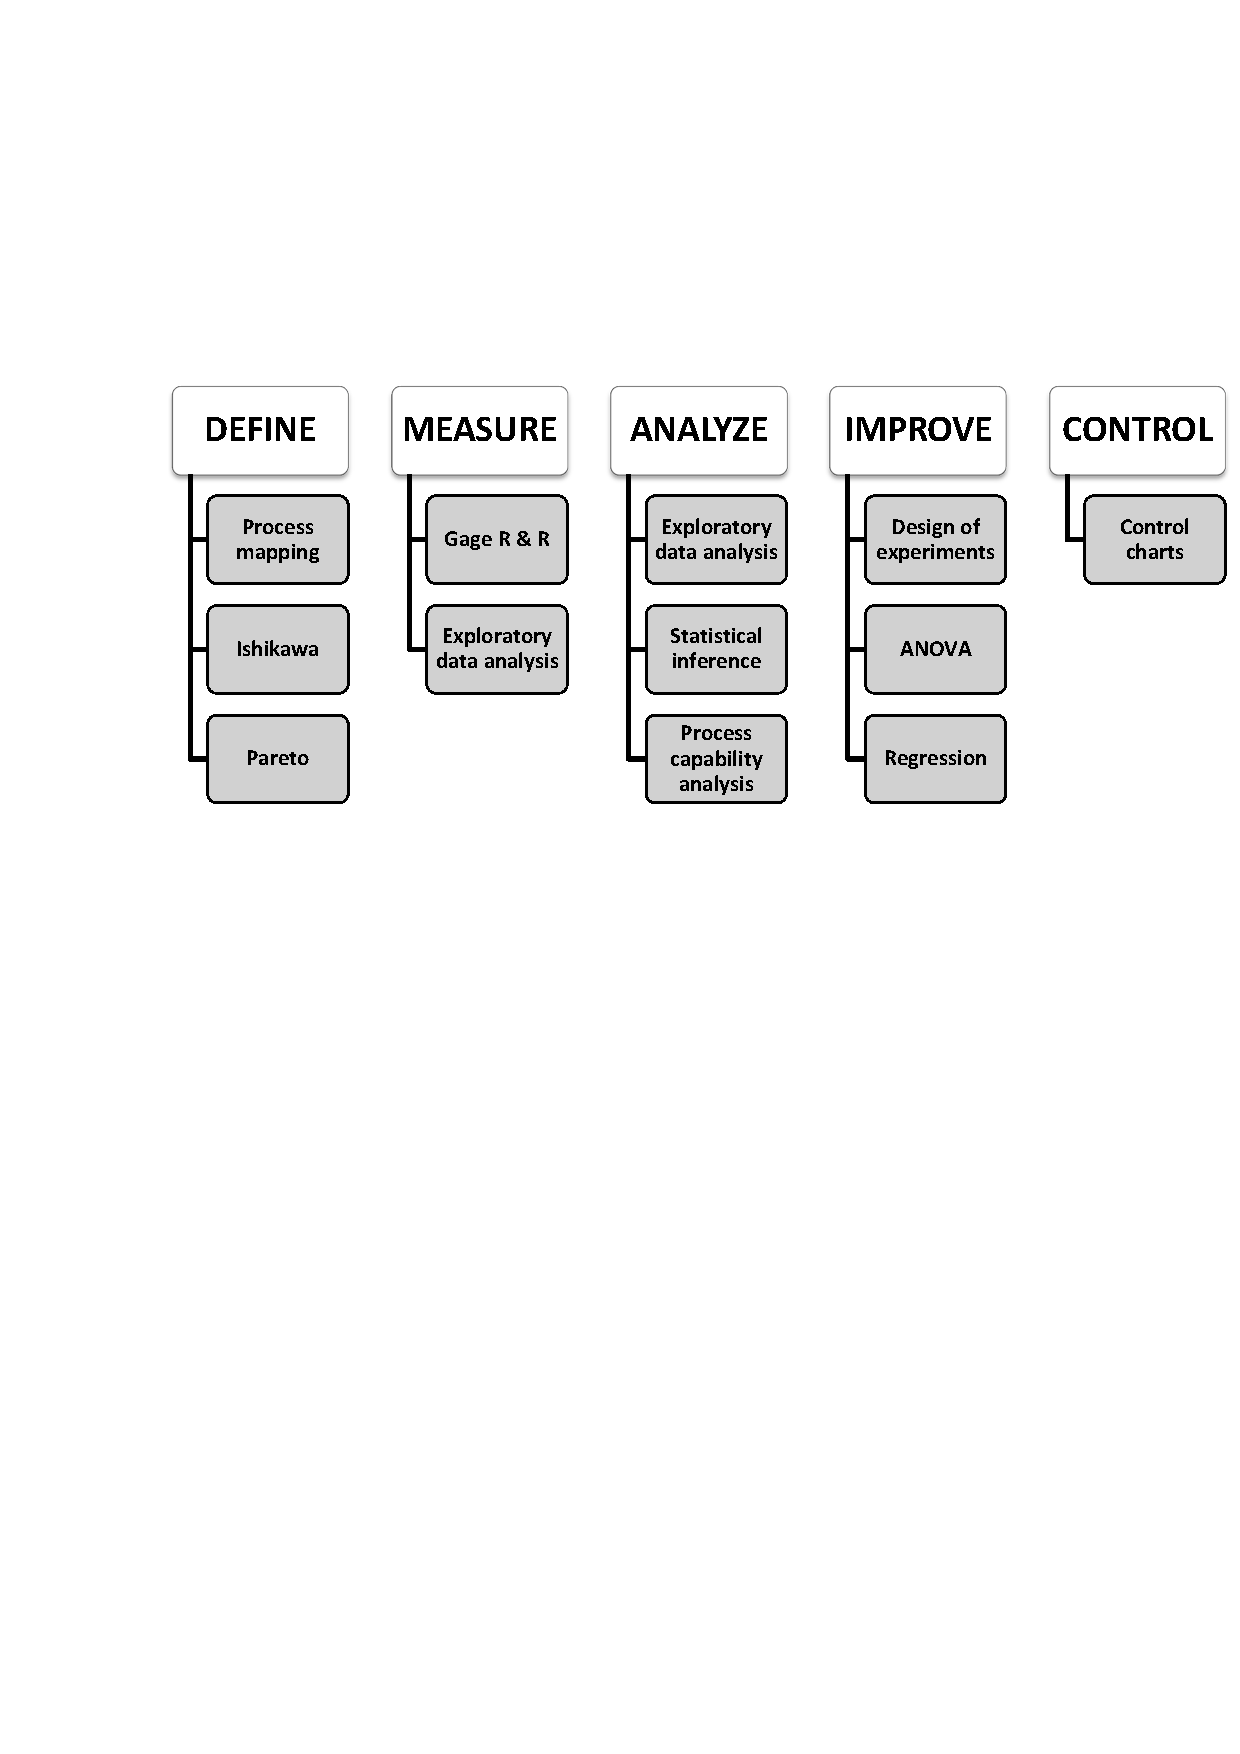
\includegraphics[width=1\linewidth]{DEMAIC.PDF}
        \caption{Statistical tools applied in each steps of the Six Sigma methodology.}
        \label{DMAIC}
	\end{figure}
    
The use of different SQC techniques was standardized With the development of the Six Sigma method by Motorola in 1997 \citep{pande2000six}. Six Sigma is a methodology or even philosophy focused on variability reduction that promotes the use of statistical methods and tools in order to improve processes in industry and services. %Six Sigma's goal is to reach maximum 3.4 defects per million of events or opportunities (DPMO) meeting the customer requirements. 
The Six Sigma application is composed of five stages: Define, Measure, Analyze, Improve, and Control (DEMAIC). 
%The Six Sigma methodology itself indicates which technique to apply at each stage of the improvement process. 
Figure~\ref{DMAIC} shows some representative statistical techniques applied in each of the Six Sigma stages. The two most representative statistical tools of SQC are the control charts and the process capability analysis \citep{montgomery2009introduction}. Therefore, the proposed \CRANpkg{qcr} package has been developed in order to provide users a comprehensive and free set of programming tools to apply control charts and perform capability analysis in the SQC framework.
\\

The control stage is characterized by the use of tools based on anomaly detection and correction \citep{montgomery2009introduction}. The most representative techniques of this stage and the primary tool of the Statistical Process Control (SPC) are the control charts \citep{champ1987exact}. They have been developed to evaluate the process performance and at any time. The use of control charts prevents the process from getting out of control, and helping to detect the assignable causes corresponding to variations of the critical-to-quality features (CTQs), thus performing process changes when actually required. Furthermore, control charts provide estimates of the natural range of process variation (natural control limits), allowing us to compare this range with those limits specified by standards, company managers, or customers (specification limits). Hence, the process monitoring can be carried out by comparing each new observation with these natural limits, preventing defects in the final product. Briefly, a control chart is a two-dimensional graph whose axis represents the variable or attribute that is being monitored (CTQ variables). %They were introduced by Shewhart in 1924 at Bell laboratories. 
The estimation of natural control limits of the CTQ variables is developed by a process composed of two phases: In Phase I, the natural control limits are estimated using a preliminary sample (calibration sample) where we assume that the causes of variation are only random. In Phase II, each new observation is plotted on the control chart along with the natural limits obtained in the previous step. The set of new observations (twhich are not used to calculate the natural control limits) make up the so-called monitoring sample. Patterns, observations of out of control limits, runs of more than six observations on one side of the central line, among others, are some of the different criteria to identify out of control states in a specific process, providing also valuable information about the detection of any assignable causes of variation in the monitoring. \\

\begin{figure}[h!]
		\centering	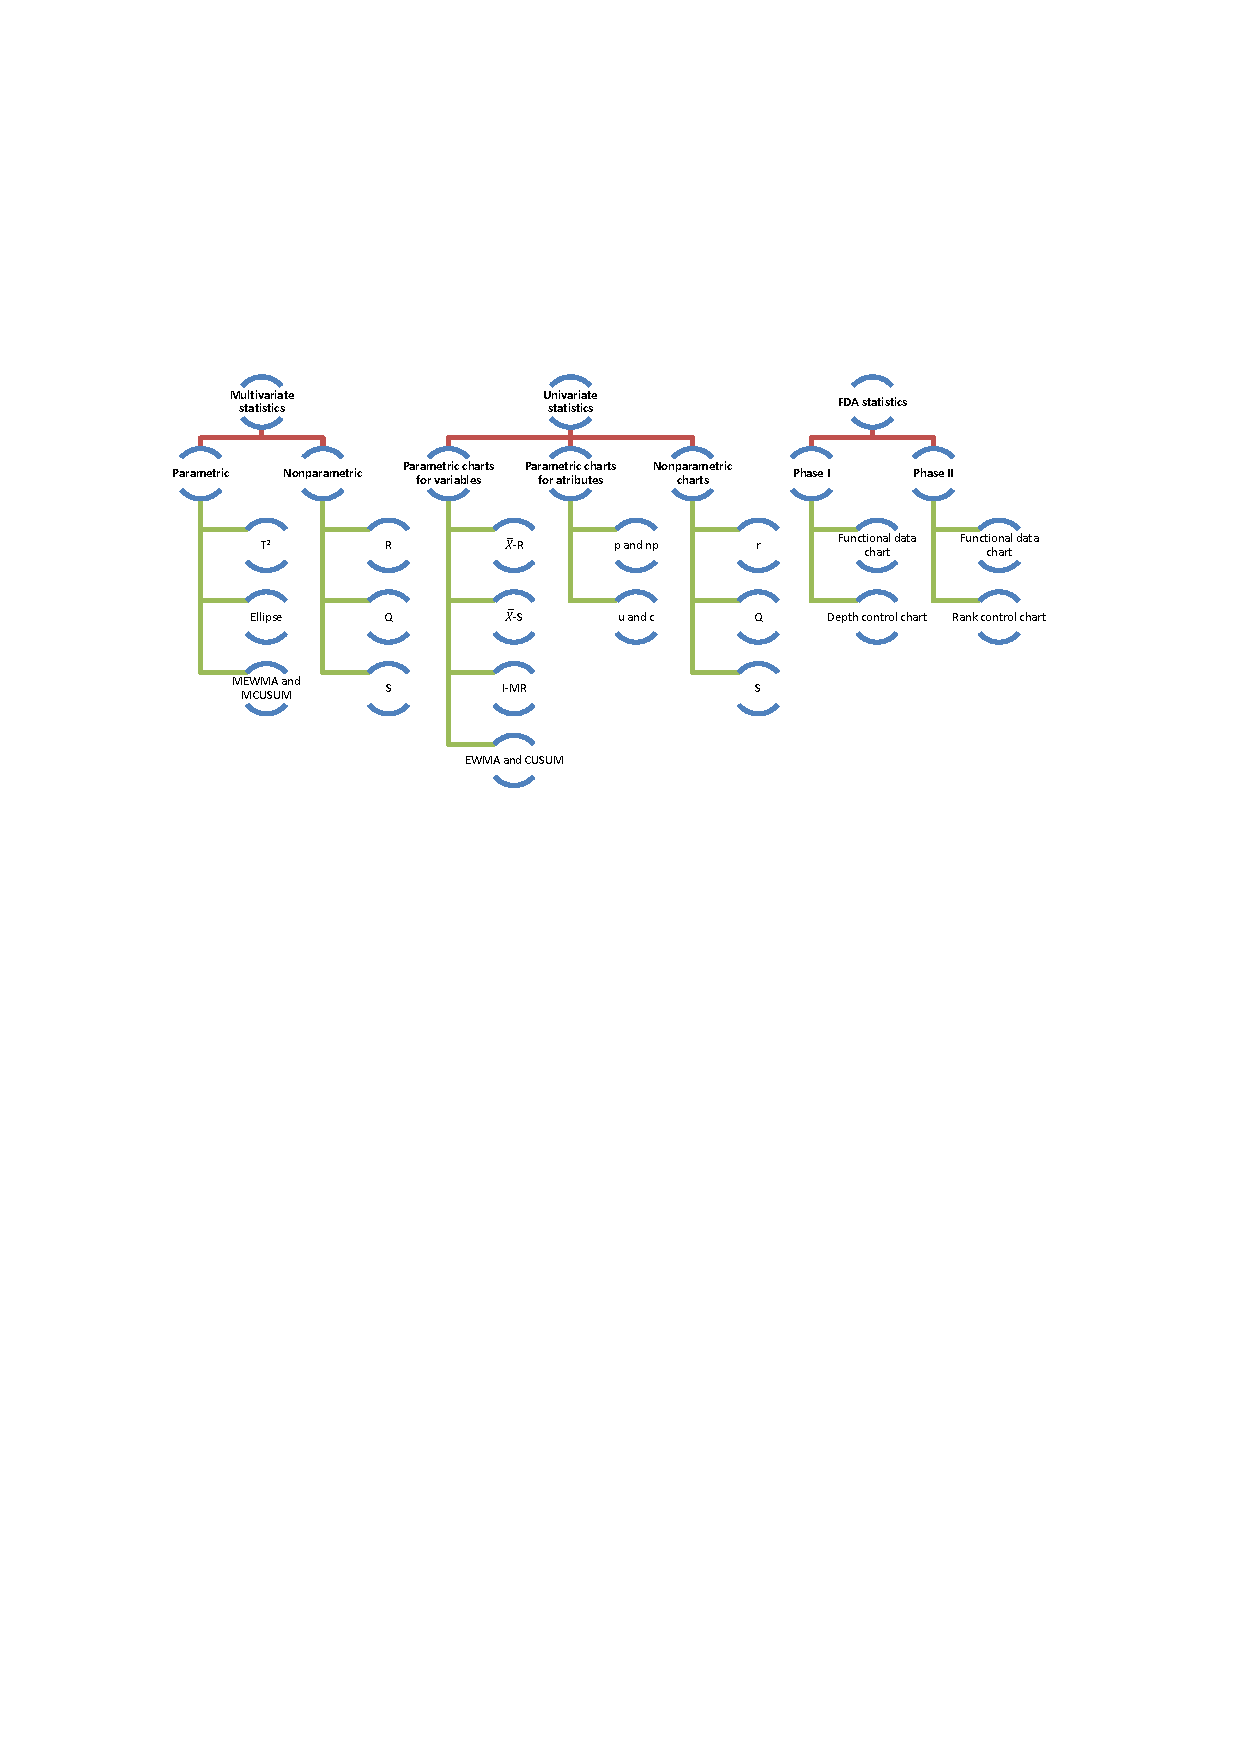
\includegraphics[width=1\linewidth]{graficos2.PDF}
        \caption{Control charts implemented in the \CRANpkg{qcr} package.}
        \label{types}
	\end{figure}
    
The most used control charts are based on the assumptions of normality and independence of the studied CTQ variables. These charts are used to control the position and dispersion of CTQ attributes and variables. Figure~\ref{types} shows some of the most important types of control charts. These can be classified according to the type of feature that is being controlled (attribute or variable), the variable dimension (univariate or multivariate), and assuming or not a parametric distribution of the variable (parametric or nonparametric). The \CRANpkg{qcr} package provides charts for the mean ($\bar{x}$), standard deviation ($s$), range ($R$), individual measurements ($I$), moving ranges ($MR$), proportion of nonconforming units ($p$), number of nonconforming units ($np$), number of defects per unit ($c$), mean number of defects per control unit ($u$), exponentially weighted moving average (EWMA), and cumulative sum control chart (CUSUM). The last two techniques are also called memory control charts, and they are specially designed to detect shifts of less than two standard deviations, both when using rational samples or individual measurements. 
On the other hand, new control charts based on the concept of data depth and developed by \cite{liu1995control} are implemented in \CRANpkg{qcr}. Those are the $r$, $Q$, and $S$ control charts, the nonparametric alternatives for individual measurements, mean control chart, and CUSUM control chart, respectively. When more than one variable defines the process quality, multivariate control charts are applied. If the Gaussian assumption is met, the Hotelling T$^2$ control chart can be applied. If we want to detect small deviations, multivariate EWMA (MEWMA) and multivariate CUSUM (MCUSUM) can be implemented. When no parametric distribution is assumed, $r$, $Q$, and $S$ charts can be used.  
\\

Another interesting SQC tool, which is very useful in the industry, is the Process Capability Analysis (PCA).
It estimates how well a process meets the tolerances defined by the company, customers, standards, etc., by comparing the specification tolerances with respect to the natural range of variation of CTQ features. The capability of the process is measured using capability indicators. Process Capability Ratio (PCR) is a numerical score that helps the manufacturers know whether the output of a process meets the engineering specifications. Large PCR values show that the industrial or service process is capable of meeting the customer requirements. There have been many different PCRs developed in the last four decades that require the Gaussian assumption for the CTQ variable \citep{boyles1991taguchi}.
However, many processes in industry and real applications do not meet this hypothesis. Thus, we could innacuratelly estimate the capability using PCR. Hence, many authors have studied different nonparametric alternatives to traditional PCR \citep{polansky2007process}. \\

%The development engine of computer applications deployed in this article is the \texttt{R} software \citep{R}. As known, \texttt{R} is a programming language and environment for statistical analysis. It is a free software project whose first steps were due to Ross Ihaka and Robert Gentleman of the Department of Statistics at the University of Auckland. However, successive versions are controlled and developed by the \texttt{R} Development Core Team which includes many partners around the world. \texttt{R} is freely distributed under the terms of the General Public License (GNU) and compiles and runs on different platforms: Unix, Windows and MacOS.\\
The \CRANpkg{qcr} package has been developed in R \citep{R} under the GNU license.
Nowadays, there are other R packages that currently provide quality control tools for users. The use of each one is shown in Figure~\ref{packages}.\\ 

The \CRANpkg{qcc} package \citep{scrucca2004qcc} was developed by Professor Luca Scrucca of the Department of Economics, Finance, and Statistics at the University of Perugia. It enables us to perform Shewhart quality control charts for variables and attributes, as well as the CUSUM and EWMA charts for detecting small changes in the CTQ variable. Multivariate analysis is performed applying the Hotelling T$^2$ control chart. Additionally, it has functions implemented to obtain the operating characteristic curves (OC) and to estimate process capability analysis indices. Pareto and Ishikawa diagrams are also implemented. Otherwise, the \CRANpkg{IQCC} package \citep{recchia2010iqcc} is maintained by Professor Emanuel P. Barbosa of the Institute of Mathematics in the State University of Campinas. It has a smaller number of control charts implemented, but it incorporates multivariate graphics. The \pkg{qualityTools} package \citep{roth2012qualitytools} was developed to aid learning in quality sciences. Figure~\ref{packages} shows some of its utilities, e.g., capability analysis (providing a comprehensive set of parametric distributions) and design of experiments. In addition, the \CRANpkg{SixSigma}  library \citep{cano2017sixsigma,cano2017sixsigma2} provides alternative functions to \pkg{qualityTools} and \CRANpkg{qcc} packages and the possibility of implementing process maps. \\

\begin{figure}[h!]
		\centering	
        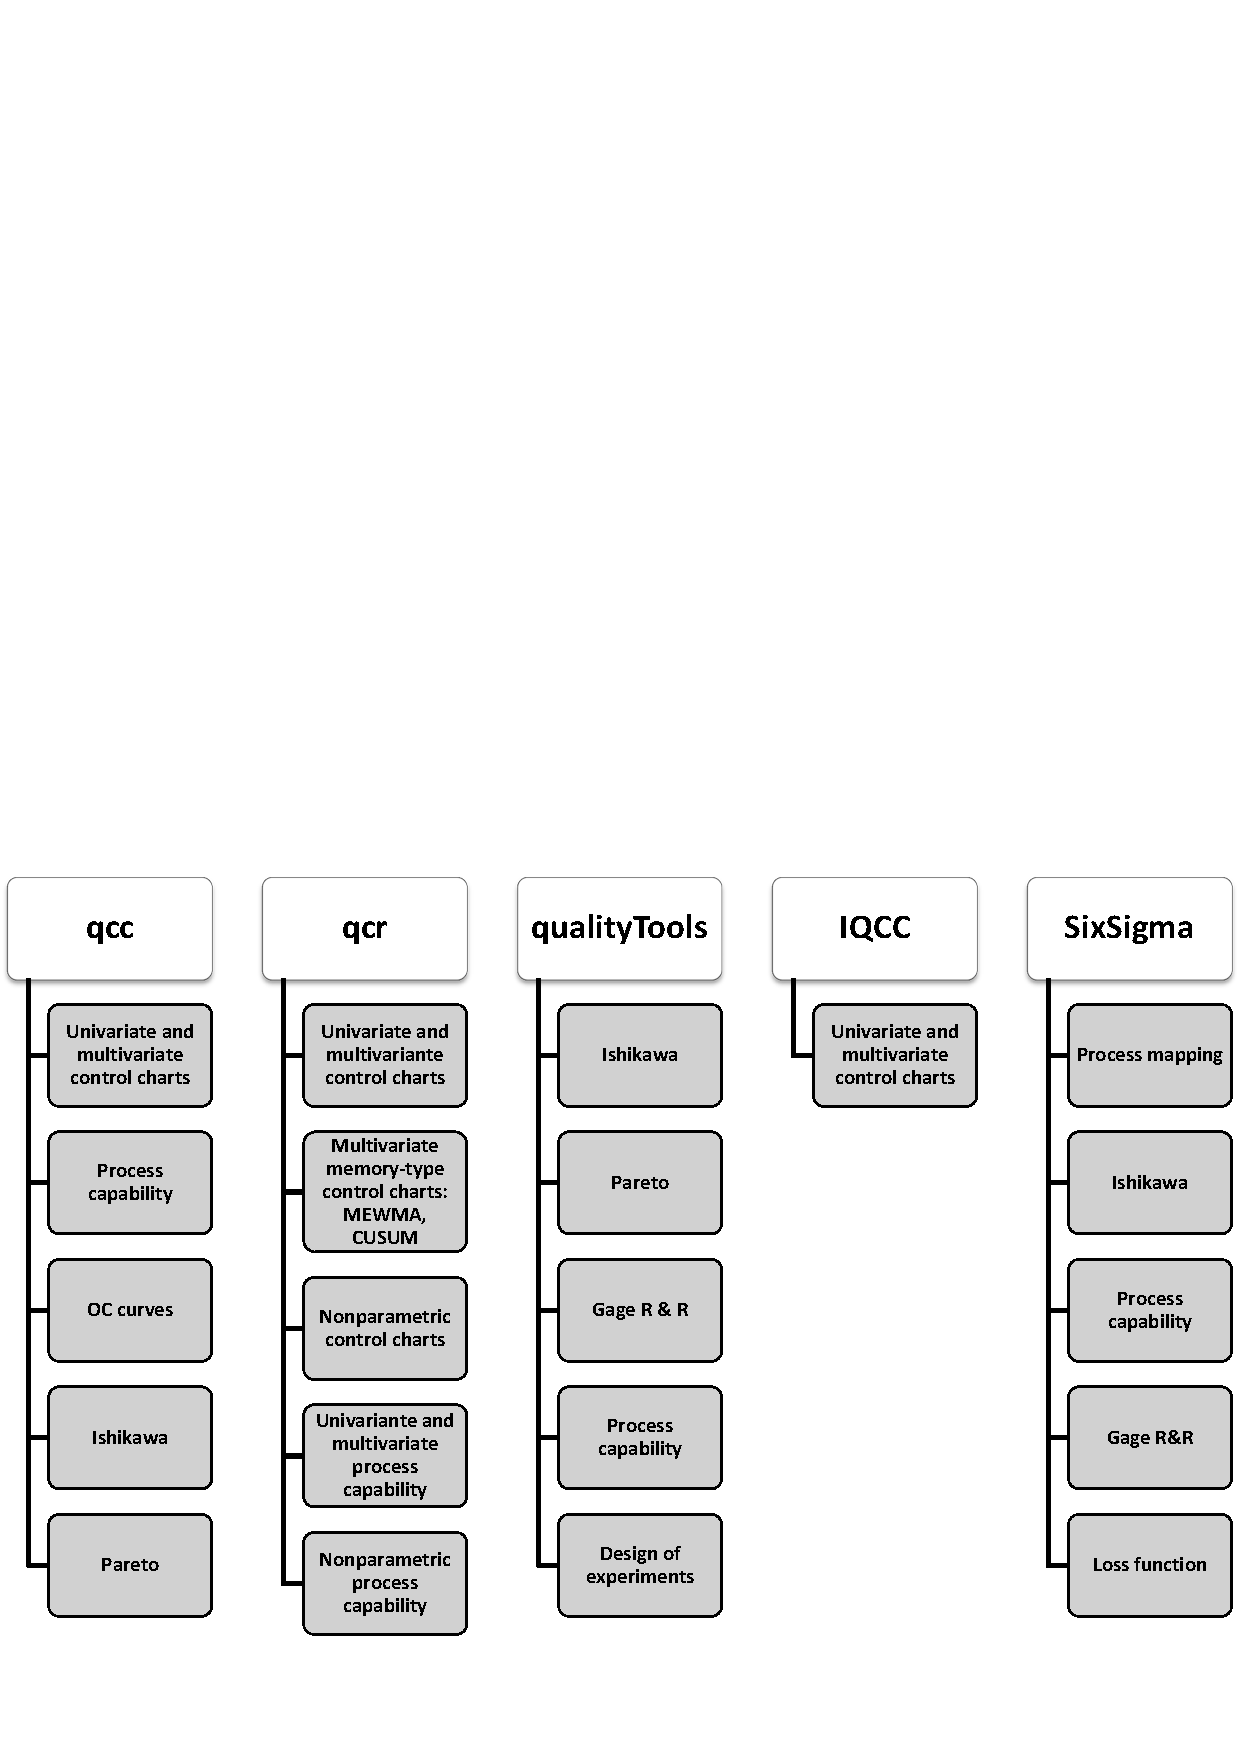
\includegraphics[width=0.80\linewidth]{packages.PDF}
        \caption{Comparison between the main packages in R devoted to Statistical Quality Control and the \CRANpkg{qcr} package.}
        \label{packages}
	\end{figure}   
    
Furthermore, there are other libraries specifically focused on control chart applications. Namely, the \CRANpkg{spcadjust} \citep{spcadjust} that allows us to estimate the calibration control limits of Shewhart, CUSUM, and EWMA control charts, and the \CRANpkg{spc} \citep{spc} which provides tools for the evaluation of EWMA, CUSUM, and Shiryaev-Roberts control charts by using Average Run Length and RL quantiles criteria. Moreover, the \CRANpkg{MSQC} package  \citep{santos2016package} is a set of tools for multivariate process control, mainly control charts. It contains the main alternatives for multivariate control charts such as Hotelling (T$^2$), Chi-squared, MEWMA, MCUSUM, and Generalized Variance control charts. It also includes some tools to evaluate the multivariate normal assumption. The corresponding multivariate capability analysis can be performed using the \CRANpkg{MPCI} library \citep{MPCI} that provides different multivariate capability indices. It is also interesting to mention the \CRANpkg{edcc} package \citep{edcc} for its economic design of control charts by minimizing the expected cost per hour of the studied process. %When  normality of data is not assumed, nonparametric graphics can be used. The \texttt{mnspc} (Nonparametric Multivariate Statistical Process Control) package \citep{bezener2011package} developed by Martin Bezener and Peihua Qiu of the University of Minnesota provides an alternative CUSUM procedure. \\

%In this article, the new \texttt{qcr} library, which implements a great deal of the statistical tools for quality control, is presented. The aim is to provide the scientific community and quality assurance users a computer application that allows simple and efficient handling of statistical tools for quality control, which are fundamental techniques in the Six Sigma methodology: control charts for variables and attributes, and capability analysis. 
It is important to emphasize that the \CRANpkg{qcr} package also includes new applications such as nonparametric approaches of control charts and capability indices (also covering the capability plots), which are currently unavailable in the R software.
%This study is composed by seven sections. The second and third shows the qcr alternatives to implement univariate a multivariate control charts, respectively. The fourth section is devoted to the applications of nonparametric control charts while the fifth one is focused on control charts for autocorrelated data. The sixth section explains how to perform capability analysis with qcr library. Finally, the main conclusions are enounced in the seventh section.


% \section{Creating a qcs object}
% 
% A \texttt{qcs} object is the starting point for control charts implementation. The required argumens are (at least) a vector containing data and a character string specifying the group statistics to compute. It allows to generate Shewhart-type charts and to obtain numerical results of interest for process quality control (involving continuous or attribute data). It also provides (see table \ref{shew}) basic functionality for univariate and multivariate (\texttt{mqcs}) quality control analysis in addition to non parametric control charts (\texttt{npqcs}) in which a depth function must be specified, as well as parametric and nonparametric process capability indices.
% 
% An object of class \texttt{qcs} is returned. Summary
% statistics can be retrieved using the \texttt{summary} function.
% 
% Its most important arguments are
% \begin{Soutput}
% qcs(x, sample.index, sizes = NULL, type = c("xbar", "R", "S", "I", "p",
%   "np", "c", "u", "ewma", "cusum"), center = NULL, std.dev, conf.nsigma = 3,
%   limits = NULL, type.data = c("continuous", "atributte", "dependence"),
%   lambda = 0.2, decision.interval = 5, se.shift = 1)
% \end{Soutput}
% 
% \texttt{qcs} quality control statistics

%-------------------------------------------
\section{Datasets in the qcr package} \label{sec:datsets}
%-------------------------------------------

The \CRANpkg{qcr} package contains new databases (see table \ref{datasets}) based on study cases tackled by the authors during their professional activity as well as well-known datasets implemented on other packages focused on statistical quality control such as: 
\begin{itemize}
\item \textbf{archery1: }It consists of a stage in which the archer shoots 72 arrows. The information is given in x and y coordinates. It is implemented in the \CRANpkg{MSQC} package (\citealt{santos2016package}).
\item \textbf{circuit: }Number of nonconformities observed in 26 successive samples of 100 printed circuit boards. It is implemented in the \CRANpkg{qcc} package (\citealt{scrucca2004qcc}).
\item \textbf{dowel1: }Diameter and length of a dowel pin. It is implemented in the \CRANpkg{MSQC} package (\citealt{santos2016package}).
\item  \textbf{orangejuice: }Frozen concentrated orange juice is packed in 6-oz cartons.  These cartons are formed on a machine by spinning them from a cardboard stock and attaching a metal bottom panel. A can is then
inspected to determine whether, when filled, the liquid could possibly leak either on the side seam or
around the bottom joint. If this occurs, a can is considered nonconforming. The data were collected
as 30 samples of 50 cans each at half-hour intervals over a three-shift period in which the machine
was in continuous operation. It is implemented in the \CRANpkg{qcc} package (\citealt{scrucca2004qcc}).
\item \textbf{pcmanufact: }A personal computer manufacturer counts the number of nonconformities per unit on the final assembly line. He collects data on 20 samples of 5 computers each. It is implemented in the \CRANpkg{qcc} package (\citealt{scrucca2004qcc}).
\item \textbf{pistonrings: }Piston rings for an automotive engine are produced by a forging process. The inside diameter of the rings manufactured by the process is measured on 25 samples, each of size 5, drawn from a process being considered `in control'. It is implemented in the \CRANpkg{qcc} package (\citealt{scrucca2004qcc}).
\end{itemize}


\begin{table}[!htb]
\centering
\begin{tabular}{ll}
\hline
\multicolumn{1}{c}{\textbf{Name}} & \multicolumn{1}{c}{\textbf{Description}} \\ \hline
\textbf{counters} & \begin{tabular}[c]{@{}l@{}}A water supply company wants to control the performance of the water\\ counters installed throughout a city. For this purpose, 60 rational\\ samples have been taken, each one  composed  by 3 measurements, from\\ the same age (10 years) and caliber water counters corresponding to\\ two different brands, and during a period of 5 years. This dataset\\ is based on a study case of A Coru\~na's water supply company, \\ Empresa Municipal de Aguas de La Coru\~na (Emalcsa).\end{tabular} \\ \hline
\textbf{employment} & \begin{tabular}[c]{@{}l@{}}A Spaniard-Argentinian hotel company wants to control the level of\\ occupancy (measured in \%) in their establishments through the\\ application of a continuous control. For this purpose, 48 subsamples have\\ been taken from six hotels corresponding to two different countries.\end{tabular} \\ \hline
\textbf{oxidation} & \begin{tabular}[c]{@{}l@{}}This database contains information about the resistance against the\\  oxidation of olive oil of the Picual variety. Five measurements of the\\ Onset Oxidation Temperature (OOT, index that measures the\\ resistance against the oxidation) are obtained from 50 batches of Picual\\ olive oil produced in chronological order. It is importantly to note\\ that OOT decreases  as the oil is progressively mixed with other\\ olive oil varieties defined by a lower OOT.\end{tabular} \\ \hline
\textbf{plates} & \begin{tabular}[c]{@{}l@{}}A chemical company is developing a patent for a new variant of artificial\\ stone mostly made of quartz (93wt\% and polyester resin). This company\\ is launching a pilot plant where it begins to produce plates of this\\ material on an industrial scale. The CTQ variable of this product is the\\ Vickers hardness. In order to measure the hardness level and hardness\\ homogeneity of the product, 50 plates have been measured 5 times in\\ different sections. The characteristic learning curves, through gradual\\ level change, can be observed.\end{tabular} \\ \hline
\textbf{presion} & \begin{tabular}[c]{@{}l@{}}A shipyard of recreational boats is intended to optimize and control the\\ mechanical properties of the yacht hulls made of a composite based on\\ epoxy resin. In this regard, the modulus of elasticity due to tensile\\ efforts is measured after applying two different curing pressures: 0.1\\ and 10 MPa. Overall, 60 subsamples, composed of three measurements,\\ obtained from 60 vessels, have been taken.\end{tabular} \\ \hline
\end{tabular}

\caption{Some of the specific datasets included in the \CRANpkg{qcr} package}
\label{datasets}
\end{table}


%-------------------------------------------
%\section{Univariate statistical quality control with Shewhart control charts}
\section{Univariate and multivariate parametric control charts in qcr}

%-------------------------------------------

%The control chart is a useful tool in statistical process control for monitoring and controlling manufacturing processes \citep{montgomery2009introduction}. It is an on-line process control technique used for detecting the occurrence of any significant process mean (or variability) change and, accordingly, calling for a corrective action. \\
The construction of a control chart is equivalent to the plotting of the acceptance regions of a sequence of hypothesis tests over time. Namely, the $\bar{x}$ chart is a control chart used to monitor the process mean $\mu$. It plots the sample means, $\bar{X}$'s, corresponding to subgroups of the  $\{X_1,X_2,...\}$ observations and is equivalent to test the hypotheses $H_0:\mu=\mu_0$ versus $H_{\alpha}:\mu \neq \mu_0$ (for some target value $\mu_0$) conducted over time, using $\bar{x}$ as the test statistic. Here we assume that $\{X_1,X_2,...\}$ are the sample measurements of a particular CTQ feature that follows the $F$ distribution with mean $\mu$ and standard deviation $\sigma$. When there is insufficient evidence to reject $H_0$, we can state that the process is under control; otherwise, the process is out of control. In other words, processes are under control when their sources of variation are only the sources common to the process \citep{brown1990statistical}. The decision to reject or not $H_0$ is based on the value of the sample mean $\bar{x}$ observed at each time interval \citep{liu1996control}.
The control charts are easy to construct, visualize, and interpret, and most important, have proven their effectiveness in practice since the 1920's.

%-------------------------------------------
%\subsection{Definition of univariate quality control objects and statistics}
%-------------------------------------------
Control charts are defined, on the one hand, by a center line that represents the average value of the CTQ feature corresponding to the in-control state and, on the other hand, two horizontal lines, called the upper control limit (UCL) and the lower control limit (LCL). The region between the control limits corresponds to the region where $H_0$ is not rejected (defined in the previous section). As a consequence, the process will be out of control when an observed rational sample or an individual measurement falls outside the limits. 
%This suggests that the studied process may have been affected by some special or assignable causes, out of the common ones. Even although all the observations (rational samples or individual measurements) were inside the control limits, the process could be out of control if the points which represent them in the control chart follow systematic patterns. Consequently, different methods such as the Western Electric rules have been developed in order to identify those sequences or non random patterns in a control chart, and therefore helping to detect out of control states \citep{montgomery2009introduction}. 
%In conclusion, control charts are a very useful tool to detect shifts with respect to the probability distribution that defines the state under control (and characterizes the quality level) of a process, whenever using the proper estimated control limits.\\
Let $w$ be a sample statistic that measures a quality characteristic of interest, and suppose that the mean of $w$ is $\mu_w$ and the standard deviation  of $w$ is $\sigma_w$. Then the center line, the upper control limit, and the lower control limit become:
$$\mbox{UCL}=\mu_w + L \sigma_w$$ 
$$\mbox{CL}=\mu_w$$ 
$$\mbox{LCL}=\mu_w - L \sigma_w,$$ 
where $L$ is the ``distance'' of the control limits from the center line, expressed in standard deviation units.\\
%In designing a control chart, the sample size and sampling frequency must be specified. Small shifts in the process will be detected much easier when large samples are measured. Taking large samples would be the desirable situation, but it is not feasible in many cases either from an economic point of view or by the characteristics of the process studied. The Average Run Length (ARL) allows us to choose the rational sample size and sampling frequency. It is defined by the number of rational samples that, on average, is necessary to monitor and plot in a control chart before an out of control state is identified. If the observations obtained from the CTQ feature of the process are not correlated, the ARL can be estimated using the Shewhart control charts by the expression
%$$ \mbox{ARL}=\frac{1}{p} $$
%where $p$ is the probability that any point exceed the natural control limits. The performance of the control charts can be evaluated using this equation, although sometimes it is recommended to express the control chart performance in terms of its Average Time to Signal (ATS), which is defined as 
%$$ \mbox{ATS}=ARL \times h $$
%whereby $h$ is the fixed time interval in which samples are taken.\\

\begin{table}[h!]
\centering
\begin{tabular}{lll}
\hline
 & & \multicolumn{1}{c}{\textbf{Statistical quality control charts for}}  \\ \hline
\textbf{Function} & \textbf{Chart name} & \multicolumn{1}{c}{\textbf{Variables}} \\ \hline
\code{qcs.xbar} & {$\bar{X}$} & \begin{tabular}[c]{@{}l@{}}Sample means of a continuous process variable are\\ plotted to control the process average. \end{tabular} \\
\code{qcs.R}    & {$R$}       & \begin{tabular}[c]{@{}l@{}}Sample ranges of a continuous process variable are\\ plotted to control the process variability. \end{tabular}  \\
\code{qcs.S}    & {$S$}       & \begin{tabular}[c]{@{}l@{}}Sample standard deviations of a continuous variable\\  are plotted to control the process variability.\end{tabular} \\
\code{qcs.one}  & {$I$}       & \begin{tabular}[c]{@{}l@{}}Sample values from a I chart data of a continuous\\ process variable to control the level (position)\\ of the process.\end{tabular} \\ 
 & & \multicolumn{1}{c}{\textbf{Attributes}}  \\ \hline
\code{qcs.p}    & $p$     & \begin{tabular}[c]{@{}l@{}}Proportion of nonconforming units is plotted, the \\ number of defective items follow a binomial distribution.\end{tabular}  \\
\code{qcs.np}   & $np$    & \begin{tabular}[c]{@{}l@{}}Number of nonconforming units is plotted, and the chart\\ is constructed based on the average of the process.\end{tabular} \\
\code{qcs.c}    & $c$     & \begin{tabular}[c]{@{}l@{}}Nonconformities per unit are plotted, number of defects\\ in a large population follow a Poisson distribution.\end{tabular}  \\
\code{qcs.u}    & $u$     & \begin{tabular}[c]{@{}l@{}}Average nonconformities per unit are plotted, this chart \\ does not require a constant number of units.\end{tabular}  \\
\code{qcs.g}    & $g$     & \begin{tabular}[c]{@{}l@{}}Number of non-events between events are plotted, it\\counts the number of events between rarely-occurring\\ errors or nonconforming incidents.\end{tabular} \\ 
 & & \multicolumn{1}{c}{\textbf{Attributes and variables}}  \\ \hline
\code{qcs.cusum}  & CUSUM & \begin{tabular}[c]{@{}l@{}}Cumulative sums for individual observations or for the\\ averages of rational subgroups are plotted to monitor\\ the process mean.\end{tabular}  \\
\code{qcs.ewma}   & EWMA  & \begin{tabular}[c]{@{}l@{}}The exponential weighed average of CTQ variables are\\plotted to identify small changes in the process \\(measured as rational samples or individual observations).\end{tabular} \\ 
 & & \multicolumn{1}{c}{\textbf{Multivariate control charts}}  \\ \hline
\code{mqcs.t2}  & T$^2$ & \begin{tabular}[c]{@{}l@{}}Multivariante Hotelling T$^2$ control chart for individual\\ observations (vectors).\end{tabular}  \\
\code{mqcs.mcusum}  & MCUSUM & \begin{tabular}[c]{@{}l@{}}Multivariate Cumulative Sum control chart for individual\\ observations (vectors).\end{tabular}  \\
\code{mqcs.ewma}   & MEWMA  & \begin{tabular}[c]{@{}l@{}}Multivariate EWMA control chart for individual\\ observations (vectors).\end{tabular} \\
 & & \multicolumn{1}{c}{\textbf{Functional data control charts}}  \\ \hline
\code{fdqcs.depth}  & Phase I & \begin{tabular}[c]{@{}l@{}}Phase I control chart for functional data:\\ depth control chart and deepest curves envelope.\end{tabular}  \\
\code{fdqcs.rank}  & Phase II & \begin{tabular}[c]{@{}l@{}}Phase II control chart for functional data:\\ rank control chart and deepest curves envelope.\end{tabular}  \\
\code{plot.fdqcs}   & FDA plots  & \begin{tabular}[c]{@{}l@{}}Graphical outputs for Phase I and Phase II control charts\\ for functional data.\end{tabular} \\ \hline
\end{tabular}
    \caption{Univariate Shewhart, multivariate Hotelling T$^2$, univariate and multivariate CUSUM and EWMA and FDA control charts available in the \CRANpkg{qcr} package}
    \label{shew}
\end{table}

When several random variables characterize the quality of a process/service, applying statistical multivariate quality control techniques becomes necessary. In fact, if we analyze each variable separately, the probability that an observation of a variable will fall within the calculated limits when it is known that the process is actually under control will no longer be 0.9973 for $6\sigma$ amplitude. Assuming independence, it will be $0.9973^p$, where $p$ is the number of CTQ features, while the probability of type I will actually lead to $\alpha'=1-(1-\alpha)^p$. Therefore, the control limits are different from those drawn, assuming the control of each CTQ variable independently from the others. Moreover, if the variables are dependent, the calculation of $\alpha$ becomes more complex. This subject is particularly important today, as automatic inspection procedures make it customary to measure many parameters of each product over time. %\citep{montgomery2009introduction}. 
The more common multivariate parametric control charts are the Hotelling T$^2$ (to identify big shifts) and the multivariate CUSUM (MCUSUM) and EWMA (MEWMA) for identifying small shifts.


The functions that compute the quality control statistics for the different univariate control charts (involving continuous, attribute or count data) are shown in Table \ref{shew}. For the sake of simplicity and taking into account that these types of control charts are implemented in other packages, the use of these functions is not shown in this work. More details are given in the help of \CRANpkg{qcr} package \citep{flores2016qualityreview}.

%\subsection{Statistical quality control with Shewhart control charts}
%Control charts can also be divided into two categories. If the CTQ feature of a specific process can take an infinite number of values in a continuous interval, it is called variable, and the corresponding charts are named control charts for variables. Otherwise, if the CTQ feature is not measured in a continuous scale, namely we only can tag each unit of product either as conforming or nonconforming on the basis of whether or not it possesses certain attributes, or alternatively we may count the number of nonconformities (defects) appearing on a unit of product, we are talking about attributes and attribute control charts.\\
%In order to illustrate the use of the \texttt{qcr} package, control charts for variables and attributes will be plotted, the construction of control limits will be specified in each section.\\
%The first steps are loading both the package and the dataset 
%
%\begin{Schunk}
%\begin{Sinput}
%R> library("qcr")
%R> data("pistonrings")
%\end{Sinput}
%\end{Schunk}
%%
%The \textbf{pistorings} data frame consists of 200 observations measured in 25 samples each one of size 5. 

%%-------------------------------------------
%\subsubsection{Control charts for X-bar, R and S }
%%-------------------------------------------
%When working with CTQ variables, monitoring both their mean and variability is necessary. 
%Hence, the $\bar{x}$ chart is used to control the process mean while the process variability can be monitored with the control chart for the range, so called $R$ control chart. 
%Taking into account that the control limits of the $\bar{x}$ chart depend on the process variability estimation, it is recommended to develop the $R$ chart in advance. 
%After assessing the process is in control in terms of variability, these estimates can be used to obtain the natural control limits of the $\bar{x}$ chart in a more reliable way. 
%
%Supposing that $i=1,\dots,k$ rational samples of size $n$ are avaliable, and let $R_i$ be the range of the $i$th sample. 
%The center line and control limits of the $R$ chart are as follows:\\
%
%\noindent$LCL = D_3 \bar{R}$\\
%$CL = \bar{R}$\\
%$UCL = D_4 \bar{R}$\\
%
%whereby $D_4$ and $D_3$ are constants tabulated for different values of $n$ \citep{montgomery2009introduction}, 
%and $\bar{R} = \frac{1}{k} \sum_i R_i$ is the average of the $k$ ranges. 
%In \texttt{R}, these control limits, as well as the center line, are computed using the \texttt{qcs.R()} function, 
%and the resulting object may be printed by using the \texttt{summary} function 
%\begin{Schunk}
%\begin{Sinput}
%R> x <- droplevels(pistonrings[1:125, ])
%R> res.qcs <- qcs.R(x, data.name = "pistonrings", std.dev = "UWAVE-R")
%R> summary(res.qcs)
%\end{Sinput}
%\begin{Soutput}
%R chart for pistonrings 
%
%Summary of group statistics:
       %R          
 %Min.   :0.00800  
 %1st Qu.:0.01800  
 %Median :0.02100  
 %Mean   :0.02276  
 %3rd Qu.:0.02600  
 %Max.   :0.03900  
%
%Group sample size:  5
%Number of groups:  25
%Center of group statistics:  0.02276
%Standard deviation:  0.009785039 
%
%Control limits: 
 %LCL        UCL
   %0 0.04812533
%
%Number beyond limits: 0 
%
%Number violationg runs: 0 
%\end{Soutput}
%\end{Schunk}
%The corresponding chart can be generated with the \texttt{plot()} method
%\begin{Schunk}
%\begin{Sinput}
%R> plot(res.qcs, title = "Control chart for pistonrings: R")
%\end{Sinput}
%\end{Schunk}
%(see Figure~\ref{fig:R}). As there are not patterns, runs, nor samples out of the natural control limits, 
%the process is assumed under control in terms of variability.
%
%\begin{figure}[!htb]
%\begin{center}
%\includegraphics{article-R-plot2}
%\caption{$R$ control chart.}
%\label{fig:R} 
%\end{center}
%\end{figure}
%
%Once the variability is controled, $\sigma$ can be estimated by using its unbiased estimator $\hat{\sigma} = \frac{1}{d_2} \bar{R}$, 
%where $d_2$ is a constant tabulated for various sample sizes \citep{montgomery2009introduction}. 
%Consequently, the process mean can be controled by an $\bar{x}$ chart, considering the $3\sigma$ control limits \\
%
%\noindent$LCL = \bar{\bar{x}}-\frac{3}{\sqrt{n}d_2}\bar{R}=\bar{\bar{x}}-A_2\bar{R}$ \\
%$CL = \bar{\bar{x}}$ \\
%$UCL = \bar{\bar{x}}+\frac{3}{\sqrt{n}d_2}\bar{R}=\bar{\bar{x}}+A_2\bar{R}$\\
    %
%where $\bar{\bar{x}}= \frac{1}{k} \sum_i \bar{x}_i$ is the global mean. 
%The null hypothesis of process in control is tested by assessing if each $\bar{x}_i$ is within the interval $[LCL, UCL]$.
%Assuming the measured variable is Gaussian and that the process is under control, the probability a point being within the natural control limits is 0.9973.
%In \texttt{R}, function \texttt{qcs.xbar()} can be applied to compute the center line and the control limits using the range for estimating the theoretical standard deviation. 
%The corresponding chart can be generated with the \texttt{plot()} method 
%\begin{Schunk}
%\begin{Sinput}
%R> res.qcs <- qcs.xbar(x, data.name = "pistonrings", std.dev = "UWAVE-R")
%R> plot(res.qcs, title = expression(paste("Control chart for pistonrings: ", 
%+    bar(x))))
%\end{Sinput}
%\end{Schunk}
%(see Figure~\ref{fig:xbar}). As shown, there is no evidence that indicates the process is out of control.
%
%\begin{figure}[!htb]
%\begin{center}
%\includegraphics{article-xbar-plot2}
%\caption{$\bar{x}$ control chart using the sample range to estimate the natural control limits.}
%\label{fig:xbar} 
%\end{center}
%\end{figure}
%
%The process standard deviation can also be  estimated using the sample standard deviation instead of the sample range. 
%This leads to control charts for $\bar{x}$ and $s$, where $s$ is the sample standard deviation, 
%and to apply the $s$ control chart instead of the $R$ chart, whose center line and control limits are\\
%
%\noindent$LCL = B_3 \bar{s}$\\
%$CL = \bar{s}$\\
%$UCL = B_4 \bar{s}$\\
%
%whereby $B_3$ and $B_4$ are tabulated constants which depend on $n$ \citep{montgomery2009introduction}, 
%and $\bar{s}= \frac{1}{k}\sum_i s_i$ is the average of the $k$ standard deviations.
%For this purpose, the \texttt{qcs.S} function can be used in \texttt{R}.
%
%In this case, assuming that variability is controlled, $\sigma$ is estimated by using its unbiased estimator
%$\hat{\sigma}= \frac{1}{c_4}\bar{s}$. 
%The $3\sigma$ natural control limits for monitoring the process mean are\\
%
%\noindent$LCL = \bar{\bar{x}}-\frac{3}{\sqrt{n}c_4}\bar{s}=\bar{\bar{x}}-A_3\bar{s}$\\    
%$CL = \bar{\bar{x}}$\\    
%$UCL = \bar{\bar{x}}+\frac{3}{\sqrt{n}c_4}\bar{s}=\bar{\bar{x}}+A_3\bar{s}$\\
%
%\noindent which also can be programmed in \texttt{R} by using the \texttt{qcs.xbar()} function, specifying \texttt{std.dev = "UWAVE-SD"} to use the sample standard deviation. 
%
%
%%-------------------------------------------
%\subsubsection{p and np control charts}
%%-------------------------------------------
%The $p$ and $np$ charts are the more representative types of atribute control charts. If $k$ random samples of $n$ items are avaliable, and denoting with $X_i$ the number of defective items in each sample, assuming that an item is nonconforming with probability $p$ and also that the items successively produced are independent, the nonconfomities follow a binomial distribution with mean $np$ and standard deviation $\sqrt{np(1-p)}$. 
%Alternatively, the sample nonconforming item fraction $\hat{p}_i= X_i / n$ has mean $p$ and standard deviation $\sqrt{p(1-p) / n}$. In both cases the asymptotic distribution is normal, from which the center line and control limits of the Shewhart chart can be worked out. For the $p$ control chart, they are given by:
%
%\noindent$LCL = \bar{p}-3\sqrt{\frac{\bar{p}(1-\bar{p})}{n}}$\\    
%$CL = \bar{p}$\\    
%$UCL = \bar{p}+3\sqrt{\frac{\bar{p}(1-\bar{p})}{n}}$\\
%
%\noindent where $\bar{p}=\frac{1}{k}\sum_i \hat{p}_i$ is the estimate of the unknown propability $p$.
%
%To illustrate the computation of the $n$ control charts, the \texttt{orangejuice} dataset \citep{scrucca2004qcc} (described in Section \ref{datasets}) will be considered. 
%The \texttt{qcs.p()} function can be used to compute statistics required for the $p$ chart. It can be directly applied to the data
%\begin{Schunk}
%\begin{Sinput}
%R> data("orangejuice")
%R> res.qcs <- qcs.p(orangejuice[orangejuice$trial, 1:2], 
%+    sizes = orangejuice$size[orangejuice$trial])
%\end{Sinput}
%\end{Schunk}
%or alternatively, a \texttt{qcd} object (quality control data) could be created first
%\begin{Schunk}
%\begin{Sinput}
%R> datos.qcd <- qcd(data = orangejuice[orangejuice$trial, ], var.index = 1, 
%+    sample.index = 2, sizes = orangejuice$size, type.data = "atributte")
%R> res.qcs <- qcs.p(datos.qcd)
%R> plot(res.qcs, title = "Control chart for orangejuice: p")
%\end{Sinput}
%\end{Schunk}
%The resulting chart is shown in Figure~\ref{fig:p}. Samples 6 and 20 are outside the control limits and should be removed from the control limit calculations since assignable causes have been found. Namely, sample 6 was examined by an inexperienced inspector who overlooked several types of nonconformities. In addition, the large number of nonconformities in sample 20 was due to a problem of temperature control in the welding machine \citep{montgomery2009introduction}.\\
%
%\begin{figure}[!htb]
%\begin{center}
%\includegraphics{article-qcs-plot}
%\caption{\label{fig:p} $p$ control chart for \texttt{oranjuice} data.}
%\end{center}
%\end{figure}
%
%If the objective is to analyze the average number of nonconformities rather than their proportion, the $np$ charts can be used. The statistics for this chart can be computed in \texttt{R} with the \texttt{qcs.np()} function. There are other alternatives to perform control of attributes such as the $c$ and $u$ charts, based on Poisson distribution. The $c$ chart controls the total number of defects per unit, whereas the $u$ chart controls the average number of nonconformities per unit. Both can be computed with the \texttt{qcr} package as shown in \cite{flores2016qualityreview}.
%
%%-------------------------------------------
%\subsubsection{CUSUM chart}
%%-------------------------------------------
%Cumulative sum control charts (CUSUM), proposed by \cite{page1954continuous} to monitor the process mean, may now be developed both for individual observations and for the averages of rational subgroups. Its use is specially recommended to identify changes less than $2\sigma$. The $s_r$ statistic is used to determine whether the process is in control or not. It is defined by
%$$s_r=\sum_{i=1}^{r}(\bar{x}_i-\mu_0)$$
%, whereby $\mu_0$ is the target for the process mean. 
%Under Gaussian assumption, the center line and control limits of the chart can be deduced from
%$s_r \sim  N\left( r(\mu-\mu_0), \frac{r\sigma_0^2}{n} \right)$.
%Considering again the \texttt{pistorings} dataset, this chart can be analogously generated 
%\begin{Schunk}
%\begin{Sinput}
%R> res.qcd <- qcd(pistonrings, type.data = "dependence")
%R> res.qcs <- qcs.cusum(res.qcd, type = "cusum")
%R> plot(res.qcs, title = "Control chart for pistonrings: CUSUM")
%\end{Sinput}
%\end{Schunk}
%and is shown in Figure~\ref{fig:CUSUM}.
%
%\begin{figure}[!htb]
%\begin{center}
%\includegraphics{article-CUSUM-plot}
%\caption{CUSUM control chart for pistonrings dataset.}
%\label{fig:CUSUM} 
%\end{center}
%\end{figure}
%
%%-------------------------------------------
%\subsubsection{EWMA control chart}
%%-------------------------------------------
%The exponentially weighted moving average (EWMA) control chart was introduced by \cite{roberts1959control} as an alternative when we are interested in detecting small shifts. The performance of the EWMA control chart is approximately equivalent to that of the cumulative sum control chart since both monitor the process mean.\\
%Both individual observations and rational sample means can be controlled by this type of chart, where moving averages $y_i$ are calculated by weighing the prior observations as follows 
%
%$$y_i=\lambda x_i+(1-\lambda)y_{i-1}$$
%
%with $0<\lambda \leq 1$ and $y_0=\mu_0$, the target. Therefore, the EWMA control chart is performed by plotting $y_i$ versus the sample number $i$ (or time). The center line and control limits for the EWMA control chart are
%
%\noindent$LCL = \mu_0-3\sigma\sqrt{\frac{\lambda(1-(1-\lambda)^{2i})}{2-\lambda}}$\\    
%$LCS = \mu_0$\\    
%$UCL = \mu_0+3\sigma\sqrt{\frac{\lambda(1-(1-\lambda)^{2i})}{2-\lambda}}$
    %
%If the value of $i$ is high, then the control limits are:
%
%\noindent$LCL = \mu_0-3\sigma\sqrt{\frac{\lambda}{2-\lambda}}$\\    
%$LCS = \mu_0$\\    
%$UCL = \mu_0+3\sigma\sqrt{\frac{\lambda}{2-\lambda}}$
    %
%The EWMA control chart is plotted and its corresponding statistics are estimated by using the  \texttt{qcs.ewma()} function in the same manner as the CUSUM chart \citep[see][]{flores2016qualityreview}.
%
 %
%%-------------------------------------------
%\subsection{Example of applying control charts to control the mean}
%%-------------------------------------------
%
%The methodology to control the central trend of a CTQ variable through the application of the Phase I and II control charts is shown in this section. The case study corresponding to the \texttt{pistorings} dataset, with piston diameter as CTQ variable, is used for this purpose.
%
%\subsubsection{Stabilizing the process and estimating the natural control limits}
%The process to estimate the natural control limits is detailed in this section. The control limits can only be estimated in a proper way when the process is stabilized, i.e., in control. If the aim is to estimate the control limits of the piston diameter from the first forty rational samples (calibration sample) is intended, the Shewhart $\bar{x}$ control chart can be developed through the code:
%\begin{Schunk}
%\begin{Sinput}
%R> pistonrings.qcd <- qcd(pistonrings)
%R> res.qcs <- qcs.xbar(pistonrings.qcd)
%R> plot(res.qcs, title = "Xbar control chart for pistonrings I")
%\end{Sinput}
%\end{Schunk}
%\begin{figure}[!htb]
%\begin{center}
%\includegraphics{article-xbar1-plot}
%\caption{$\bar{x}$ control chart (first step)}
%\label{fig:xbar1}
%\end{center}
%\end{figure}
%(see Figure~\ref{fig:xbar1}), and the results can be printed by calling
%\begin{Schunk}
%\begin{Sinput}
%R> summary(res.qcs)
%\end{Sinput}
%\begin{Soutput}
%xbar chart for pistonrings 
%
%Summary of group statistics:
      %xbar      
 %Min.   :73.99  
 %1st Qu.:74.00  
 %Median :74.00  
 %Mean   :74.00  
 %3rd Qu.:74.01  
 %Max.   :74.02  
%
%Group sample size:  5
%Number of groups:  40
%Center of group statistics:  74.0036
%Standard deviation:  0.01007094 
%
%Control limits: 
      %LCL      UCL
 %73.99009 74.01712
%
%Beyond limits of control: 
%[1] 74.0196 74.0234
%
%Violationg runs: 
%[1] 74.0128
%\end{Soutput}
%\end{Schunk}
%(the sample range is used to estimate the variance by default). Figure~\ref{fig:xbar1} shows that two points are out of the control limits and another point is within the limits but corresponds to a run, therefore the process is out of control \cite{woodall2000controversies}. The next step, once the assignable causes of these shifts are identified, is to remove the points that fall out the control limits (in red) and also the runs (in orange) and after recalculate the control limits until the process is in control. The \texttt{qcr} library includes the \texttt{state.control()} function that removes the points indicative of out-of-control state and also returns a \textit{qcd} object used to build a new control chart.
%\begin{Schunk}
%\begin{Sinput}
%R> res.qcd <- state.control(res.qcs)
%R> res.qcs <- qcs.xbar(res.qcd)
%R> plot(res.qcs, title = "Xbar control chart for pistonrings II")
%\end{Sinput}
%\end{Schunk}
%\begin{figure}[!htb]
%\begin{center}
%\includegraphics{article-xbar2-plot}
%\caption{$\bar{x}$ control chart (second step)}
%\label{fig:xbar2}
%\end{center}
%\end{figure}
%Figure~\ref{fig:xbar2} still shows a point outside the control limits. Therefore, the \texttt{state.control()} function is used to delete it and the control limits are estimated again. Figure~\ref{fig:xbar3} shows that the process is under control, thus, the control limits estimates are reliable.
%\begin{Schunk}
%\begin{Sinput}
%R> res.qcd <- state.control(res.qcs)
%R> res.qcs <- qcs.xbar(res.qcd)
%R> plot(res.qcs, title = "Xbar control chart for pistonrings III")
%\end{Sinput}
%\end{Schunk}
%\begin{figure}[!htb]
%\begin{center}
%\includegraphics{article-xbar3-plot}
%\caption{$\bar{x}$ control chart (second step)}
%\label{fig:xbar3}
%\end{center}
%\end{figure}
%
%
%%-------------------------------------------
%\subsubsection{Monitoring a process}
%%-------------------------------------------
%When the process is under control (Phase I) and once the control limits are calculated, the process is monitored (Phase II). In the next case, the first 25 subsamples (more than 20 are recommended) of piston diameter are used as calibration sample in order to estimate the control limits, whereas the remaining subsamples of \texttt{pistonrings} dataset form the monitoring sample. It is important to stress they are not taken into account in the natural control limits calculation \citep[see][]{montgomery2009introduction}. In Phase II, the hypothesis that each new observation belongs to the distribution of the CTQ variable estimated in Phase I is tested. Figure~\ref{fig:monitor1} shows the control limit estimation through the calibration sample. The process described by the diameter of pistons is in control. The corresponding code is:
%
%\begin{Schunk}
%\begin{Sinput}
%R> x <- droplevels(pistonrings[1:125, ])
%R> y <- droplevels(pistonrings[126:200, ])
%R> res.qcs <- qcs.xbar(x, data.name = "Xbar control chart for pistonrings")
%R> plot(res.qcs)
%\end{Sinput}
%\end{Schunk}
%\begin{figure}[!htb]
%\begin{center}
%\includegraphics{article-monitor1-plot}
%\caption{Phase I example.}
%\label{fig:monitor1}
%\end{center}
%\end{figure}
%
%
%Once the control limits are obtained, the remaining samples are monitored (Figure~\ref{fig:monitor2}) by running
%\begin{Schunk}
%\begin{Sinput}
%R> res.qcs <- qcs.add(x = res.qcs, value = y[, 1:2])
%R> plot(res.qcs)
%\end{Sinput}
%\end{Schunk}
%\begin{figure}[!htb]
%\begin{center}
%\includegraphics{article-monitor2-plot}
%\caption{Phase II example.}
%\label{fig:monitor2}
%\end{center}
%\end{figure}
%As Figure~\ref{fig:monitor2} suggests, the process falls out of control from sample number thirty seven onwards, where the diameters are unusually high when compared with the calibration sample counterparts. These four points form a bunch pattern whose assignable cause should be identified before making any corrective actions or even recalculating the control limits due to an actual change in the process.
%
%%-------------------------------------------
%\subsubsection{Warning limits}
%%-------------------------------------------
%Warning limits are applied during the Phase II when using the Shewhart control charts, in order to improve their performance against small shifts. They can be defined with a semi-amplitude of about $2\sigma$ as shown in Figure~\ref{fig:warning}. 
%\begin{Schunk}
%\begin{Sinput}
%R> res.qcs <- qcs.xbar(x, data.name = "Xbar control chart for pistonrings")
%R> plot(res.qcs, conf.nsigma.alert = 2)
%\end{Sinput}
%\end{Schunk}
%\begin{figure}[!htb]
%\begin{center}
%\includegraphics{article-warning-plot}
%\caption{Warning limits.}
%\label{fig:warning}
%\end{center}
%\end{figure}
%
%However, the ARL is reduced when the process is actually in control. To prevent this drawback, CUSUM and EWMA control charts are excellent alternatives to the Shewhart control chart for detecting small changes (less than $2\sigma$) during the Phase II of the process monitoring.

%%-------------------------------------------
%\section{Multivariate statistical quality control}
%%-------------------------------------------
%
%When several random variables characterize the quality of a process/service, applying statistical multivariate quality control technique becomes necessary. In fact, if we analyze each variable separately, the probability that an observation of a variable will fall within the calculated limits when it is known that the process is actually under control, will no longer be 0.9973 for $6\sigma$ amplitude. Assuming independence, it will be $0.9973^p$, where $p$ is the number of CTQ features, while the probability of type I will actually lead to $\alpha'=1-(1-\alpha)^p$.\\
%Therefore, the control limits are different from those drawn assuming the control of each CTQ variable independently from the others. Moreover, if the variables are dependent, the calculation of $\alpha$ becomes more complex. This subject is particularly important today, as automatic inspection procedures make it customary to measure many parameters of each product over time. %\citep{montgomery2009introduction}.

%%-------------------------------------------
%\subsection{Definition of multivariate quality control objects and statistics}
%%-------------------------------------------
%In order to perform multivariate SQC, some some definitions are needed. Thus, suppose a random sample obtained from a multivariate normal distribution, $(\mathbf{x}_1,\mathbf{x}_2,\ldots,\mathbf{x}_n)$, whereby the $i$th component contains observations on each of the $p$ variables, $x_{i1},x_{i2},...,x_{ip}$. Then, the \textit{sample mean vector} is
%$$\bar{\mathbf{x}} = \frac{1}{n}\sum_{i=1}^n\mathbf{x_i} 
%= (\bar{x}_1,\bar{x}_2,\ldots,\bar{x}_p)$$
%and the \textit{sample covariance matrix} is
%$$S=\frac{1}{n-1}\sum_{i=1}^n(\mathbf{x_i}-\mathbf{\bar{x}})(\mathbf{x_i}-\mathbf{\bar{x}})^\top $$
%with 
%$$s_{jk}=\frac{1}{n-1}\sum_{i=1}^n(x_{ij}-\bar{x}_j)(x_{ik}-\bar{x}_k) $$
%The sample mean vector and sample covariance matrix are unbiased estimators of the corresponding population parameters, i.e.,
%$$E(\mathbf{\bar{x}})=\boldsymbol{\mu} = (\mu_1,\ldots,\mu_p) \ \ \mbox{and} \ \ E(S)=\Sigma$$

%This section uses the \texttt{dowel1} dataset (composed of two CTQ variables, diameter and length of a dowel pin, that characterize its manufacturing process) available in the \texttt{MSQC} package. This data set is first transformed into an array by using the \texttt{mqcd()} function of the \texttt{qcr} library
%\begin{Schunk}
%\begin{Sinput}
%R> data("dowel1")
%R> data.mqcd <- mqcd(dowel1)
%\end{Sinput}
%\end{Schunk}

%%-------------------------------------------
%\subsection{Statistical control using the $T^2$, MCUSUM and MEWMA charts}
%%-------------------------------------------
%\subsubsection{Hotelling $T^2$ control chart}
%%-------------------------------------------
%The Hotelling $T^2$ control chart is the most popular tool devoted to control the quality of processes and services from more than one CTQ variable. 
%Consider a control process in which $p$ variables are observed and distributed according to $p$-variant normal distribution $\mathcal{N}_p(\boldsymbol{\mu}_0,\Sigma_0)$ with a vector of means $\boldsymbol{\mu}_0=(\mu_{01},\mu_{02},...,\mu_{0p})$ and a variance-covariance matrix $\Sigma_0$ of order $p$. 
%We want to test the hypothesis: $H_0:\boldsymbol{\mu}_i=\boldsymbol{\mu}_0, \forall i$ vs $H_1:\exists \boldsymbol{\mu}_j \neq \boldsymbol{\mu}_0$,  to determine if the process is under control.
%For this purpose, different criteria have been developed, highlighting the $T^2$ Hotelling statistic, defined as
%$$T^2_i=n\left( \bar{\mathbf{x}}_i-\boldsymbol{\mu}_0\right)^\top \Sigma_0^{-1}\left( \bar{\mathbf{x}}_i-\boldsymbol{\mu}_0\right)$$
%whereby $\bar{\mathbf{x}}_i=\left( \bar{x}_{i1},\dots,\bar{x}_{ip}\right)$ is the vector of means for the $p$ characteristics in the $i$th subsample. 
%When the subgroup size is one, vectors of observations will be obtained instead of vectors of means. 
%When the process is under control $(\boldsymbol{\mu}_i=\boldsymbol{\mu}_0)$, there is a probability $\alpha$, that the $T^2_i$ statistic exceeds the critical value $\mathcal{X}^2_{p,\alpha}$. Therefore, a value of the $T^2_i$ statistic exceeding the $\mathcal{X}^2_{p,\alpha}$ value is taken as an out of control signal. \\
%From a geometric point of view, the $T^2$ statistic is the ratio of the squared  distance (Mahalanobis) between a multivariate observation and the vector of target values (vector of means), where equidistant points form ellipsoids around that vector of means. The greater the value of $T^2$, the greater the distance between the observation and the target value.\\
%If $\boldsymbol{\mu}_0$ and $\Sigma_0$ are known and the process is under control, the $T^2_i$ statistic is distributed as a central chi-squared with $p$ degrees of freedom ($T^2_i \sim \mathcal{X}^2_p$).
%When the process is out-of-control, the statistic is distributed as a non central chi-squared with $p$ degrees of freedom and non-centrality parameter 
%$\lambda = n\left( \boldsymbol{\mu}_1-\boldsymbol{\mu}_0\right)^\top \Sigma_0^{-1}\left( \boldsymbol{\mu}_1-\boldsymbol{\mu}_0\right)$, where $\boldsymbol{\mu}_1$ is the mean vector of the $p$ characteristics when there is a changein at least one of the $d$ means.\\
%In practice, the value of the $T^2$ statistic is estimated by the corresponding sample values through the expression
%$$ T^2=n\left( \bar{\mathbf{x}}-\bar{\bar{\mathbf{x}}}\right)^\top S^{-1}\left( \bar{\mathbf{x}}-\bar{\bar{\mathbf{x}}}\right)$$
%whose distribution under the null hypothesis is
%$$T^2 \sim \frac{p\left( m-1\right) \left(n-1 \right) }{mn-m-p+1}F_{p,mn-m-p+1}$$
%Namely, in this case, the statistic follows approximately a $F$ distribution with $p$ and $(mn - m - p + 1)$ degrees of freedom. Since both the $\mathcal{X}^2$ and $F$ distributions are asymmetrical with right skewness, only the expression for the upper control limit is considered, which is given by
%$$UCL=\frac{p\left( m-1\right) \left(n-1 \right) }{mn-m-p+1}F_{\alpha,p,mn-m-p+1}$$\
%and $LCL=0$ is considered for the lower control limit.
%In addition, for processes in which $m$ is sufficiently large ($m>100$), this limit can be approximated by $UCL=\mathcal{X}^2_{\alpha,p}$.
%
%\cite{alt198817} recommend using these limits in a first phase, which is called a retrospective analysis. Once the control limit is estimated, a second control limit is estimated in the Phase II of process monitoring. Hence, a consistent change consisting on the multiplication of the UCL by $\frac{m+1}{m-1}$, thus obtaining a new value for the upper control limit.
%
%In the case of individual observations, i.e., $n = 1$, and assuming that we have overall $m$ subsamples to evaluate $p$ control variables, the corresponding control chart is developed from the following control limits
%
%\noindent$UCL=\frac{p\left( m+1\right) \left(n-1 \right) }{m^2-mp}F_{\alpha,p,m-p}$\\
%$LCL=0$
%
%The \texttt{mqcs.t2()} function can used to compute statistics required by the $T^2$ chart
%\begin{Schunk}
%\begin{Sinput}
%R> res.mqcs <- mqcs.t2(data.mqcd)
%R> plot(res.mqcs, title = "Hotelling control chart for dowel pin")
%\end{Sinput}
%\end{Schunk}
%\begin{figure}[!htb]
%\begin{center}
%\includegraphics{article-hotelling-plot}
%\caption{Hotelling $T^2$ control chart.}
%\label{fig:hotelling}
%\end{center}
%\end{figure}
%As shown in Figure~\ref{fig:hotelling}, the control limits have been estimated observing that the Dowell pins process is under control. The next step should be to implement the Phase II process monitoring using the proper UCL. The UCL for retrospective analysis or for monitoring phase can be computed by setting the \texttt{phase} argument to 1 or 2, respectively, of the \texttt{mqcs.t2()} function.
 %
%\subsubsection{MCUSUM control charts}
%%-------------------------------------------
%\citet{woodall1985multivariate} proposed a scheme based on multiple univariate CUSUM control charts. This method is often preferable to Hotelling's $T^2$ procedure for controlling those processes defined by Gaussian bivariate CTQ variables, as it also happened in the univariate approach when identifying small shifts from the mean is intended.\\
%\citet{healy1987note} developed the following multivariate CUSUM model:
%$$G_i=max\left\lbrace \left( G_{i-1}+a^\top\left( \mathbf{x}_i-\boldsymbol{\mu}_0\right)-0.5D \right),0 \right\rbrace$$
%whereby
%\begin{itemize}
%\item $\boldsymbol{\mu}_0$ is the mean vector when the process is under control,
%\item $\Sigma_0$ is variance-covariance matrix when process is under control,
%\item $\boldsymbol{\mu}_1$ acounts for the mean vector when the process is out-of-control,
%\item $D = \sqrt{\left( \boldsymbol{\mu}_1-\boldsymbol{\mu}_0\right)^\top \Sigma_0^{-1}\left( \boldsymbol{\mu}_1-\boldsymbol{\mu}_0 \right)}$ is a noncentrality parameter,
%\item $a^\top=\frac{A}{D}$ with $A=\left(\boldsymbol{\mu}_1-\boldsymbol{\mu}_0\right)^\top\Sigma_0^{-1}$.
%\end{itemize}
%In order to interpret the chart, an alarm signal is produced when $G_i$ exceeds a certain reference value $H$, conveniently chosen and tabulated. \citet{hawkins1991multivariate} developed a model for variables adjusted by multivariate regression, based on the assumption that when a change occurs in the mean, it is due to a magnitude variation in the mean of one of the variables of the multivariate dataset. Other proposed MCUSUM charts are those of \citet{crosier1988multivariate} and \citet{pignatiello1990comparisons}. The Croiser procedure has been implemented in the \texttt{qcr} package. This method reduces each multivariate observation to a scalar from which the CUSUM statistic is finally developed using the following expression:\\
%$$ S_i=max\left\lbrace0,S_{i-1}+T_i-k \right\rbrace $$
%where $T_i=\sqrt{n\left( \bar{\mathbf{x}}_i-\boldsymbol{\mu}_0\right)^\top \Sigma_0^{-1}\left( \bar{\mathbf{x}}_i-\boldsymbol{\mu}_0\right)}$, and $S_0 \geq 0$ (generally $S_0=0$) and $k>0$.\\
%The MCUSUM chart gives an out of control signal when the value of $S_i$ is greater than a certain value $h$ which depends on the value of the desired ARL when the process is operating at the target value $[S_i> h]$.
%Crosier used Markov processes for determining the values of $h$ and $k$ with $p=2,5,10 \  \mbox{and} \  20$ and ARL values of 200 and 500 (with process is under control). These tables were designed to detect a change $d = 1$ in the mean vector, where $d =\lambda$, with $\lambda$ a non-centrality parameter. % In this special case, the optimal values of $k$ approximate to $p$.\\
%The \texttt{mqcs.mcusum()} function of \texttt{qcr} package is used to compute the statistics required to perform the MCUSUM chart
%\begin{Schunk}
%\begin{Sinput}
%R> res.mqcs <- mqcs.mcusum(data.mqcd)
%R> plot(res.mqcs, title = "MCUSUM control chart for  dowel pin")
%\end{Sinput}
%\end{Schunk}
%\begin{figure}[!htb]
%\begin{center}
%\includegraphics{article-mcusum-plot}
%\caption{MCUSUM control chart.}
%\label{fig:mcusum}
%\end{center}
%\end{figure}
%Figure~\ref{fig:mcusum} indicates that the process is under control. 
%By default, the parameters $k=0.5$ and $h=5.5$ are chosen. For more information see \cite{montgomery2009introduction} and \cite{flores2016qualityreview}.
%
%\subsubsection{MEWMA control charts}
%The exponentially weighted moving average chart for the multivariate case (MEWMA) is an extension of the corresponding univariate chart. The multivariate extension, proposed by \citet{lowry1992multivariate}, is defined as
%$$Z_i=\Lambda \bar{\mathbf{x}}_i +\left( I-\Lambda\right)Z_{i-1}$$
%where $\bar{\mathbf{x}}_i$ is the mean vector and $\Lambda = diag\left( \lambda_1, \ldots, \lambda_p \right)$, where $\lambda_j$ accounts for the ``depth'' of memory for each variable, i.e., weights the importance of the previous observations for calculating each moving average. The higher the value of $\lambda_j$, the lower the depth and the importance of past observations. Further, $I$ is the identity matrix and $Z_0 = 0$ is considered as initial value.\\
%The information provided by the $Z_i$ is collected in the statistic
%$$T^2_i=Z_i^\top\Sigma_{Z_i}^{-1}Z_i$$
%Whereby $\Sigma_{Z_i}^{-1}$ is the inverse of the variance-covariance matrix of the $Z_i$.\\
%The control output signal occurs when $T^2_i$ exceeds a certain value $h > 0$, selected in order to achieve a certain ARL value when the process is in control. Usually, if there is no prior reason for weighting with different weights the previous observations of each one of the $p$ variables, $\lambda_1=\dots=\lambda_p$ is assumed.\\
%The $Z_i$ matrix can be obtained from the elements of the variance-covariance matrix corresponding to the variables analyzed by the expression
%$$\Sigma_{Z_i}=\frac{\lambda}{2-\lambda}\left[ 1-\left( 1-\lambda\right)^{2i} \right]\Sigma_x $$
%where $\Sigma_x$ is the original variance-covariance matrix.\\
%When $r=1$, the MEWMA chart matches the $T^2$ control chart since the asymptotic value of the variance-covariance matrix of $Z_i$ is
%$$\Sigma_{Z_i}=\frac{\lambda}{2-\lambda}\Sigma_x $$ 
%Regarding the choice of the upper control limit, \citet{runger1996markov} suggest a Markov chain approximation, which allows us to study the performance of the chart taking into account the ARL.
%They also provide a series of recommendations for selecting the parameters of the proposed control chart. Moreover, \citet{montgomery2009introduction} recommends the $\lambda$ parameter value to be between 0.05 and 0.25. The higher the value of the parameter, the less importance will be given to values that are further away in time. 
%Taking into account ARL based criteria, $\lambda=0.1$ is usually chosen in practical applications. 
%This is the default value when the \texttt{qcr} \texttt{mqcs.mewma()} function is used to compute statistics required by the MEWMA chart
%\begin{Schunk}
%\begin{Sinput}
%R> res.mqcs <- mqcs.mewma(data.mqcd)
%R> plot(res.mqcs, title = "MEWMA control chart for  dowel pin")
%\end{Sinput}
%\end{Schunk}
%\begin{figure}[!htb]
%\begin{center}
%\includegraphics{article-mewma-plot}
%\caption{MEWMA control chart.}
%\label{fig:mewma}
%\end{center}
%\end{figure}
%See the package documentation \citep{flores2016qualityreview} for more information about the arguments of this function. As in the previous cases, after the estimation of the corresponding control limits, the MEWMA control chart shown in Figure~\ref{fig:mewma} indicates that the process is under control.


%-------------------------------------------
\section{Nonparametric control charts based on data depth}    
%-------------------------------------------

The control charts presented in this section were proposed by \cite{liu1995control} as an alternative to those described in previous section. 
The main idea of its control graphs is to reduce each multivariate measure to the univariate index, that is, its relative center-exterior classification induced by a depth of data.  
This approach is completely nonparametric, and therefore, these control charts are not defined by any parametric assumption regarding the process model.  
Thus, they are applicable in a wider number of case studies than those counterparts such as  $T^2$, MCUSUM, and MEWMA control charts. In addition, these graphs allow the simultaneous detection of the change of location (shift of the mean) and the increase of the scale (change in variability) in a process.

\cite{liu1995control} proposed and justified three types of control charts, the $r$, $Q$, and $S$ charts which can be considered as data-depth-based multivariate generalizations of the univariate $X$, $\bar{x}$, and CUSUM charts, respectively.

%-------------------------------------------
\subsection{Data depth}
%-------------------------------------------
In multivariate analysis, the term depth refers to the degree of centrality of a point regarding a data cloud or a probability distribution. Therefore, it is possible to define a rank in the multidimensional Euclidean space through the calculation of observation depth. According to \cite{dyckerhoff2004data} and \citet{cascos2011data}, the depth function can be defined as a bounded function $D_{p}:R^{d} \longrightarrow R$, with $P$ the distribution set in $R^d$, that assigns at each point of $R^d$ its degree of centrality with respect to $P$. Depth functions with which control charts can be performed are the
\begin{itemize}
\item Simplicial depth (\citealt{liu1990notion}),
\item Mahalanobis depth (\citealt{mahalanobis1936generalised}),
\item Halfspace or Tukey depth (\citealt{tukey1975mathematics}),
\item Likelihood depth (\citealt{fraiman1997multivariate}), and
\item Random projection depth (\citealt{zuo2000general}).
\end{itemize}
%The \texttt{fda.qcr} package can be used to compute all the above mentioned depths.

\subsection{Statistics derived from data depth}
%-------------------------------------------
Let $G$ a $k$-dimensional distribution, and let $Y_1,\dots,Y_m$ be $m$ random observations from $G$. The sample $Y_1, \dots , Y_m$ is generally the reference sample of a CTQ variable in the context of quality control, composed of measurements from products obtained by an under control process. If $X_1, X_2, \dots$ are the new observations from the manufacturing process, assuming that the different $X_i$ values follow an $F$ distribution if the quality of the studied product has been deteriorated or, in other words, if the process is out of control. Otherwise, they follow a $G$ distribution. Let $D_G(\cdot)$ denote a notion of depth, and assume that $G$ and $F$ are two continuous distributions. Thus, if all the $D_G(Y_i)$ values are sorted in increasing order, and $Y_{[j]}$ denotes the sample value associated with the $j$th smallest depth value, then $Y_{\left[ 1\right]},\ldots,Y_{\left[ m\right]}$ are the order statistics of $Y_i$'s,
with $Y_{[m]}$ being the most central point. Therefore, the smaller the order (or
the rank) of a point, the farther that point will be from the underlying distribution  $G(\cdot)$.

\citet{liu1995control} defines the rank statistic as 
$$r_{G}\left( y\right)= P\left\lbrace D_{G}\left( Y\right) \leq D_{G}\left( y\right) \mid Y\sim G \right\rbrace$$ 
whereby $Y \sim G$ indicates that the random variable $Y$ follows the distribution $G$. When $G$ is unknown, the empirical distribution $G_{m}$ of the sample $\{Y_1, \ldots, Y_m\}$ can be used instead, and the statistic is defined by 
$$r_{G_{m}}\left( y\right)= \frac{ \# \left\lbrace D_{G_{m}}\left( Y_j\right) \leq D_{G_{m}}\left( y\right), j = 1,\ldots,m \right\rbrace}{m}$$
In the same way that $r_{G}$ and $r_{G_{m}}$, the $Q$ statistics can be also defined as follows

$$Q\left( G,F\right)= P\left\lbrace D_{G}\left( Y\right) \leq D_{G}\left( X\right) \mid Y\sim G, X\sim F \right\rbrace=E_{F}\left[ r_{G}\left( X\right) \right]$$

$$Q\left( G,F_{n}\right)= \frac{1}{n} \sum _{i=1}^{n} r_{G}\left( X_i\right)$$

$$Q\left( G_{m},F_{n}\right)= \frac{1}{n} \sum _{i=1}^{n} r_{G_{m}}\left( X_i\right),$$

\noindent whereby $F_n(\cdot)$ denotes the empirical distribution of the sample $\{X_1, \dots , X_n\}$.
The control charts corresponding to these statistics can be developed as described in the following sections.

\subsection{The $r$ chart}
%-------------------------------------------
Calculate $\left\lbrace r_{G}\left( X_1\right),r_{G}\left( X_2\right),\ldots,r_{G}\left( X_n\right)\right\rbrace$ or $\left\lbrace r_{G_{m}}\left( X_1\right),r_{G_{m}}\left( X_2\right),\ldots,r_{G_{m}}\left( X_n\right)\right\rbrace$ 
if $G$ is unknown but $Y_1,\ldots,Y_m$ are available. 
As a result, the $r$ chart consists of plotting the rank statistic in regard to time. 
The control chart central line is CL = $0.5$, whereas the lower limit is LCL =$\alpha$, with $\alpha$ accounting for the false alarm rate. The process will be out of control if $r_G(\cdot)$ falls under LCL. A small value of the rank statistic $r_{Gm}(X)$ means that only a very small proportion of $Y_i$ values are more outlying than $X$. Therefore, assuming that $X \sim F$, then a small value of $r_{Gm}(X)$ suggests a possible deviation from $G$ to $F$. This may be due to a shifting in the location and/or an increase in the scale of the studied CTQ variable. Taking into account that the UCL is not defined for the $r$ chart, the CL line serves as a reference to identify emerging patterns, runs, or trends. If $r_{Gm}(X)$ is greater than 0.5, there is evidence of scale decreasing, and also could take place a negligible location shift. This case should be tackled as an improvement in quality given a gain in the accuracy, and thus the process should not be considered as out of control.

\subsection{The $Q$ chart}
%-------------------------------------------
The idea behind the $Q$ chart is similar to the one behind the $\bar{x}$ chart. If $X_1, X_2, \dots$ are univariate and $G$ is a normal distribution, the $\bar{x}$ chart plots the averages of consecutive subsets of the different $X_i$. A goal of this type of chart is that it can prevent the identification of a false alarm when the process is actually in control (even when some individual sample points fall out of control limits due to random fluctuations). \\
The $Q$ chart is the nonparametric alternative to the $\bar{x}$ chart. It is performed by plotting the averages of consecutive subsets of size $n$ corresponding to the rank statistic ($r_G(X_i)$ or $r_{Gm}(X_i)$), given by $Q\left( G,F_{n}^j\right)$ or $Q\left( G_{m},F_{n}^j\right)$, whereas $F_n^j$ is the empirical distribution of the $X_i$'s in the $j$th subset, $j =1, 2, \dots$. Accordingly, if only $\left\lbrace Y_1, Y_2,\ldots, Y_m \right\rbrace$ are available, the $Q$ chart plots the sequence $\left\lbrace Q\left( G_{m},F_{n}^j\right),Q\left( G_{m},F_{n}^j\right),\ldots\right\rbrace$.\\
Depending on the value of $n$, the corresponding control limits are as follows:
\begin{itemize}

\item If $n \geq 5$, $CL = 0.5$ and 

  \begin{itemize}
  
    \item $LCL = 0.5-Z_{\alpha}\left( 12n\right)^{\frac{1}{2}}$ for $Q\left( G,F_{n}^j\right)$.

    \item $LCL = 0.5-Z_{\alpha}\sqrt{\frac{1}{12}\left(\frac{1}{m}+\frac{1}{n}\right)}$ 
    for $Q\left( G_m,F_{n}^j\right)$.
  
  \end{itemize}

\item If $n < 5$, $CL = 0.5$ and $LCL = \frac{\left( n!\alpha\right)^{\frac{1}{n}}}{n}$.

\end{itemize}

\subsection{The $S$ control chart}
%-------------------------------------------
The $S$ control chart is based on the CUSUM univariate control chart, 
which is basically the plot of $\sum_{i=1}^{n}\left( X - \mu \right)$, which reflects the pattern of the total deviation from the expected value. 
As mentioned above, it is more effective than the $X$ chart or the $\bar{x}$ chart in detecting small process changes. 
The nonparametric CUSUM chart based on data depth suggests plotting $S_n(G)$ and $S_n(G_m)$, defined by 
$$S_n\left( G\right) = \sum_{i=1}^{n}\left( r_G\left( X_i\right)  - \frac{1}{2} \right)$$ 
with control limits $CL = 0$ and $LCL = -Z_{\alpha}\left(\frac{n}{12}\right)^{\frac{1}{2}}$ and
$$S_n\left( G_m\right) = \sum_{i=1}^{n}\left( r_{G_{m}}\left( X_i\right)  - \frac{1}{2} \right).$$
If only $Y_1, \dots Y_m$ are available, the control limits are $CL = 0$ and $LCL = -Z_{\alpha}\sqrt{n^2\frac{\left(\frac{1}{m}+\frac{1}{n}\right)}{12}}$.
The LCL control limits in both cases constitute a curve instead of a straight line; if $n$ is large, the control chart $S$ should be standardized as follows:
$$S_n^{*}\left( G\right) = \frac{S_n^{*}\left(G\right)}{\sqrt{\frac{n}{12}}}$$
$$S_n^{*}\left( G_m\right) = \frac{S_n\left(G_m\right)}{\sqrt{n^2\frac{\left(\frac{1}{m}+\frac{1}{n}\right)}{12}}}$$
Therefore, this $S^*$ chart is defined by $CL = 0$ and $LCL = -Z_{\alpha}$.

%-------------------------------------------
\subsection{Examples of $r$, $Q$ and $S$ control charts applied using synthetic data}
%-------------------------------------------
A bivariate data set is used to illustrate how the previously discussed control charts arise.
In fact, a synthetic dataset composed of 540 observations of a bidimensional standard Gaussian variable has been 
simulated, in addition to 40 individuals corresponding to another bidimensional Gaussian variable with mean 
and standard deviation equal to 2.
\begin{example}
R> mu <- c(0, 0)
R> Sigma <- matrix(c(1, 0, 0, 1), nrow = 2)
R> Y <- rmvnorm(540, mean = mu, sigma = Sigma)
R> u <- c(2, 2)
R> S <- matrix(c(4, 0, 0, 4), nrow = 2)
R> x <- rmvnorm(40, mean = u, sigma = S)
\end{example}

Prior to the application of nonparametric control charts, the dataset has to be converted into a \code{npqcsd} object.
The synthetic dataset is arranged as two matrices, \code{G} composed of the 500 first rows (multivariate observations) of \code{Y}, 
and \code{x} with the remaining ones and including those belonging to the second bidimensional variable 
\begin{example}
R> x <- rbind(Y[501:540, ], x)
R> G <- Y[1:500, ]
R> data.npqcd <- npqcd(x, G)
\end{example}
In the same way, the \code{npqcd} function creates a data object for non parametric quality control, 
the \code{npqcs.r()}, \code{npqcs.Q()}, and \code{npqcs.S()} functions computes all the statistics required to obtain the $r$, $Q$, and $S$ control charts, respectively. 
The argument \code{method = c("Tukey", "Liu", "Mahalanobis", "RP", "LD")} specifies the data depth function, and \code{alpha} is the signification level that defines the LCL. 
See \cite{flores2016qualityreview} to obtain additional information about these functions and their arguments.

\subsubsection{$r$ chart}
%-------------------------------------------
The $r$ control chart can be obtained by applying the \code{npqcs.r()} function to the \code{npqcd} object and plotting the result.
\begin{example}
R> res.npqcs <- npqcs.r(data.npqcd, method = "Tukey", alpha = 0.025)
R> plot(res.npqcs, title = " r Control Chart")
\end{example}
The resulting chart is shown in  Figure~\ref{fig:rchart}, where it can be observed that the process is out of control from the 42nd observation, as expected, taking into account that most of the $r_{Gm}(X_i$) values are falling below the LCL.
\begin{figure}[!htb]
\begin{center}
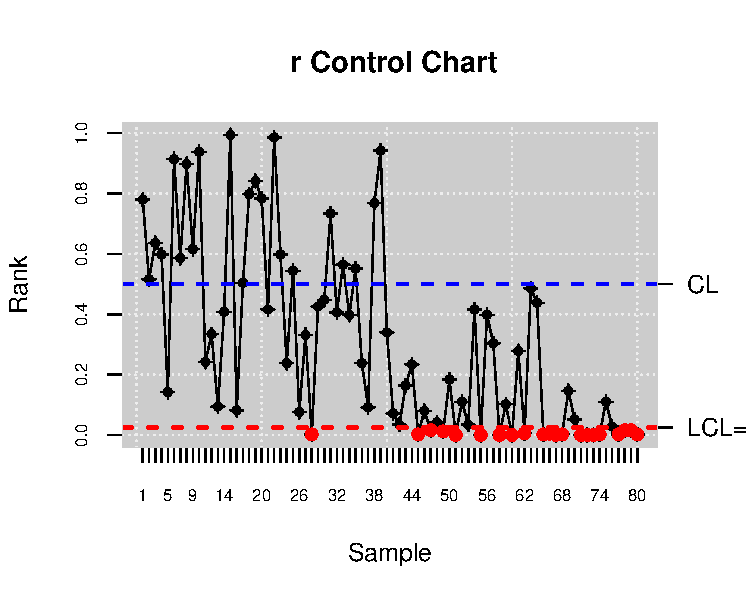
\includegraphics[width=0.8\textwidth]{article-rchart-plot}
\caption{$r$ control chart.}
\label{fig:rchart}
\end{center}
\end{figure}

\subsubsection{$Q$ chart}
%-------------------------------------------
In this case, the dataset is assumed to be composed of rational samples of size 4. 
Thus, the $Q$ nonparametric alternative of $\bar{x}$ chart is proposed and applied to control the bidimensional process:
\begin{example}
R> n <- 4    # samples
R> m <- 20   # measurements
R> k <- 2    # number of variables
R> x.a <- array( , dim = c(n, k, m))
R> for (i in 1:m) {
+      x.a[, , i] <- x[(1 + (i - 1) * n):(i * n), ]
+  }
R> data.npqcd <- npqcd(x.a, G)
R> res.npqcs <- npqcs.Q(data.npqcd, method = "Tukey", alpha = 0.025)
R> plot(res.npqcs, title = "Q Control Chart")
\end{example}
Figure~\ref{fig:Qchart} clearly shows that the process is out of control in the second half, from the 20th rational sample. 
We can also see that the high random fluctuations of the $r$ chart are attenuated in the $Q$ chart due to the averaging effect.
\begin{figure}[!htb]
\begin{center}
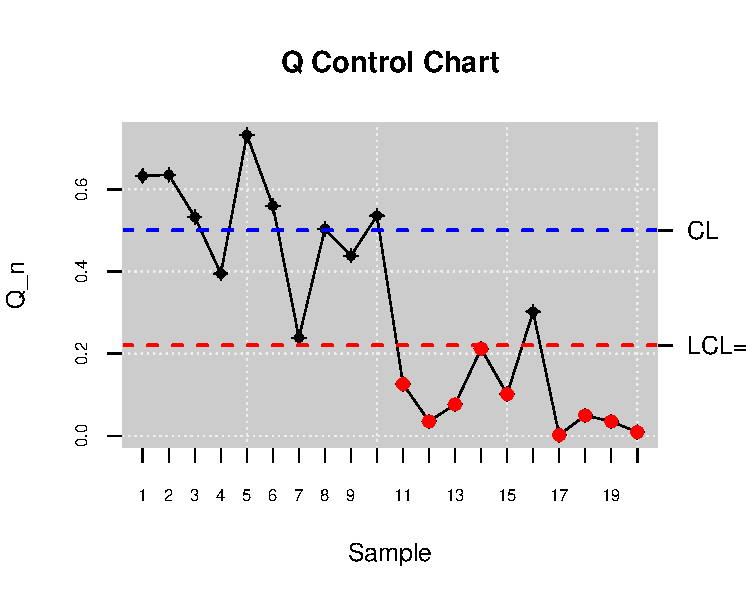
\includegraphics[width=0.8\textwidth]{article-Qchart-plot}
\caption{$Q$ control chart.}
\label{fig:Qchart}
\end{center}
\end{figure}


\subsubsection{$S$ chart}
%-------------------------------------------
Finally, the nonparametric counterpart of CUSUM control chart is performed from the multivariate individual observations.
\begin{example}
R> data.npqcd <- npqcd(x, G)
R> res.npqcs <- npqcs.S(data.npqcd, method = "Tukey", alpha = 0.05)
R> plot(res.npqcs, title = "S Control Chart")
\end{example}
Figure~\ref{fig:Schart} shows that the process is out of control from the 48th observation.  
Note that the $S$ graph performs better in identifying small changes in a process. 
In this case, the performance of the $Q$ chart is better than the corresponding to the $S$ chart. 
\begin{figure}[!htb]
\begin{center}
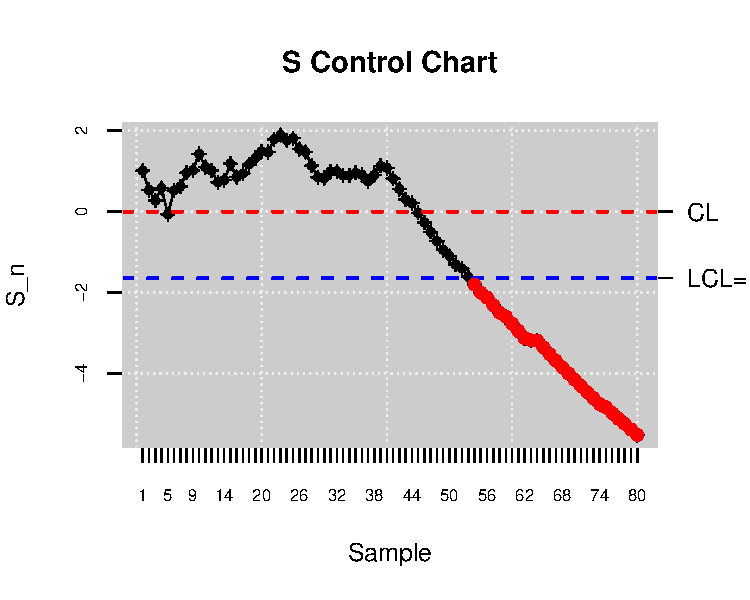
\includegraphics[width=0.8\textwidth]{article-Schart-plot}
\caption{$S$ control chart.}
\label{fig:Schart}
\end{center}
\end{figure}

%-------------------------------------------
\subsection{Control charts for functional data based on data depth}
%-------------------------------------------

In the paradigm of Industry 4.0, processes and services are many times described by continuously monitored data of hourly, daily, monthly curves or smooth functions. When the processes are defined by functional data, the authors encourage to apply control charts based on Functional Data Analysis (FDA) in order to implement control and improvement tasks. In this section, the use of control charts presented in Flores et al. \citep{flores2020constructing}. Summarizing, this methodology consists of the proposal of new Phase I and Phase II control charts to be applied in those case study in which the datum unit is a curve. Phase I control chart is based on the computation of functional data depth (specifically Fraiman and Muniz \citep{fraiman2001trimmed}, Mode \citep {cuevas2007robust}, and random projections \citep{cuevas2007robust} data depth) from which a data depth control chart is developed. Once the in-control calibration sample is obtained, the Phase II control chart based on functional data depth and rank nonparametric control chart can be applied. In addition to the Phase I functional data depth and Phase II rank control charts, plots of functional envelopes from the original curves are provided in order to help to identify the possible assignable causes of out of control states.

\subsubsection{Estimating a Phase I control chart for functional data (calibration)}

A dataset is simulated in order to illustrate the use of FDA control charts for Phase I and II. A functional mean, $mu_0$, and a functional standard deviation, \code{sigma}, are defined as shown in \citep{flores2020constructing}. An $n_0=100$ hundred curves composed of $m=30$ points are simulated. They account for the calibration or retrospective sample.


\begin{example}
R> library(fda.usc)
R> m <- 30
R> tt<-seq(0,1,len=m)
# H0
R> mu_0<-30 * tt * (1 - tt)^(3/2)
R> n0 <- 100
R> mdata<-matrix(NA,ncol=m,nrow=n0)
R> sigma <- exp(-3*as.matrix(dist(tt))/0.9)
R> for (i in 1:n0) mdata[i,]<- mu_0+0.5*mvrnorm(mu = mu_0,Sigma = sigma )
\end{example}

Prior to the application of control charts, the dataset is converted in a specific format by the \code{fdqcd} function. A plot function is also programmed to properly show the original functional data, \code{plot.fdqcd}. Figure \ref{fig:fda_1} shows the original functional data consisting of curves.

\begin{example}
R> fdchart <- fdqcd(mdata)
R> plot(fdchart,type="l",col="gray",main="Functional data")
\end{example}


\begin{figure}[!htb]
\begin{center}
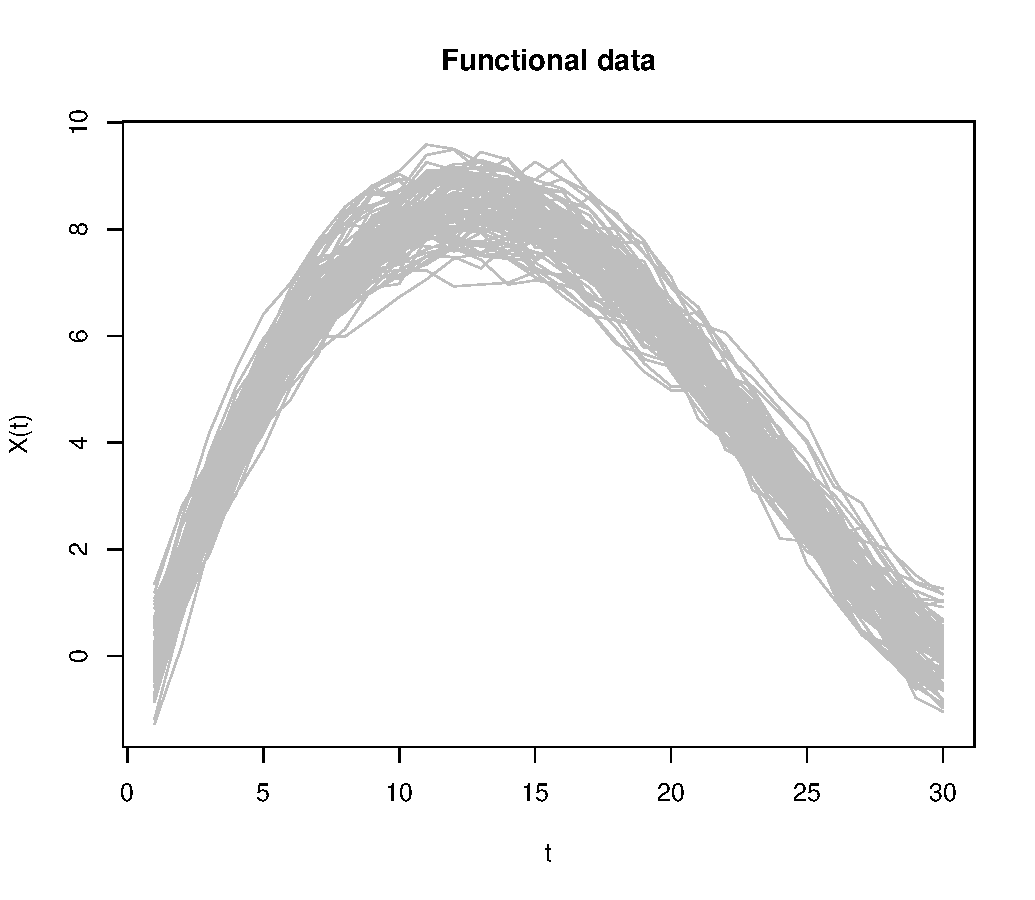
\includegraphics[width=\textwidth]{fda_1}
\caption{Original curves that account for the calibration sample.}
\label{fig:fda_1}
\end{center}
\end{figure}

The following step is to identify those curves that account for the in-control process. This task is done by the application of a Phase I control chart for functional data. This method is implemented in the \CRANpkg{qcr} package by the \code{fdqcs.depth} function. Specifically, the arguments and default values for these functions are 

\begin{example}
R> fdqcs.depth.default <- function(x, data.name=NULL,func.depth = depth.mode,nb=200,
+                                 type = c("trim","pond"),ns =  0.01, 
+                                 plot = TRUE, trim = 0.025, smo =0.05,
+                                 draw.control = NULL,...)
\end{example}

\noindent where \code{func.depth} is the type of depth measure, by default \code{depth.mode}, \code{nb} the number of bootstrap resamples, \code{type} accounts for the method used to trim the data, \code{trim} or \code{pond} \citep{flores2020constructing}, \code{ns} is the quantile to determine the cutoff from the bootstrap procedure \citep{flores2020constructing}, \code{plot} a logical value indicating that it should be plotted, \code{trim} the percentage of the trimming, \code{smo} the smoothing parameter for the bootstrap resampling \citep{flores2020constructing}, whereas \code{draw.control} specifies the \code{col}, \code{lty}, and \code{lwd} for the fdataobj, statistic, IN and OUT objects. When the \code{fdqcs.depth} function is applied to the curves of the calibration sample, the \code{fddep} object of \code{fdqcs.depth} class is obtained. It is composed of the original data, the depth corresponding to each curve, the lower control limit of the depth chart, the index of those curves out of control, the curves that account for the limits of the envelope composed by the deepest cures, and the deepest curve or functional median.


\begin{example}
R> fddep <- fdqcs.depth(fdchart)
R> summary(fddep)
\end{example}
\begin{example}
      Length Class  Mode   
fdata 100    fdata  list   
Depth 100    -none- numeric
LCL     1    -none- numeric
out     1    -none- numeric
fmin    1    fdata  list   
fmax    1    fdata  list   
fmed    1    fdata  list   
ns      1    -none- numeric
\end{example}
\begin{example}
R> class(fddep)
\end{example}
\begin{example}
[1] "fdqcs.depth"
\end{example}
\begin{example}
R> plot(fddep,title.fdata = "FDA chart",title.depth = "Depth chart")
R> out <- fddep$out; out
\end{example}
\begin{example}
[1] 29
\end{example}


Figure \ref{fig:fda_2} shows the control chart for the depth of the curves (right panel). The LCL is estimated by a smoothed bootstrap procedure \citep{flores2020constructing}. In order to provide a tool to identify the assignable cause of each out-of-control curve, the original curves with the envelope with the 99\% of the deepest curves are also shown (left panel). The analysis of the shape and magnitude of the curves in and out of bounds  can help to associate each curve out of control to an assignable cause, allowing for processes control, maintenance, and improvement.

\begin{figure}[!htb]
\begin{center}
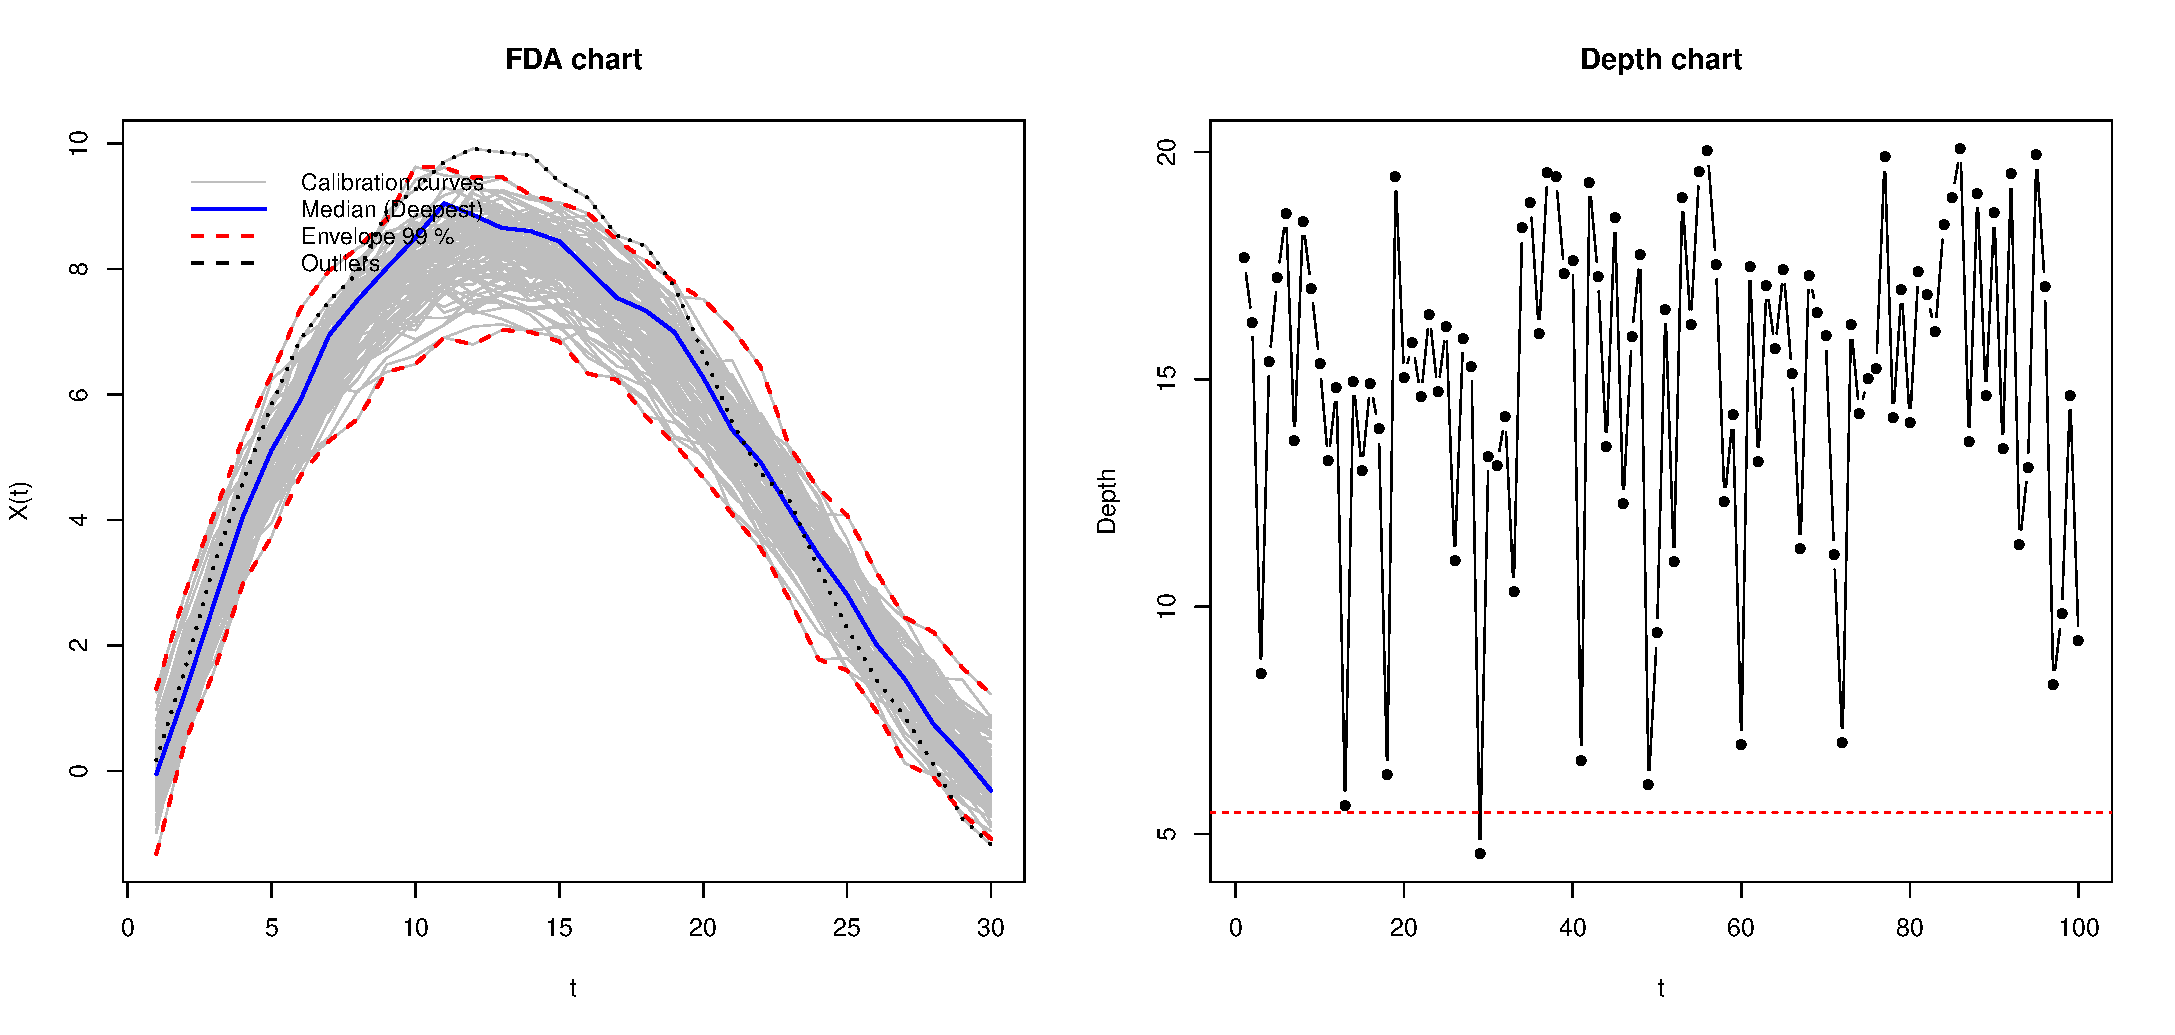
\includegraphics[width=\textwidth]{fda_2}
\caption{Left panel: Original curves with the envelope composed of 90\% of the deepest curves. Right panel: Control chart for the depths of the curves (the LCL has been estimated by bootstrap procedures at a signification level of 10\%.}
\label{fig:fda_2}
\end{center}
\end{figure}

Phase I ends when a calibration sample without curves out of control is obtained. The iterative procedure to obtain an in control calibration sample is shown in the following lines.

\begin{example}
R> alpha <- 0.1
R> trim <- 0.1
R> while (length(out)>0) {
R>   mdata <- fddep$fdata$data[-out,]
R>   fddep <- fdqcs.depth(mdata,ns = alpha, trim=trim, plot=FALSE)
R>   out <- fddep$out
R> }
R> plot(fddep,title.fdata = "Envelope with the 90\% deepest curves",
+  title.depth = "Depth control chart")
\end{example}

Figure \ref{fig:fda_3} is obtained from the application of \code{plot} function to \code{fddep} object. It shows that all the curves of the calibration sample are in control, and thus, the natural variability of the process is estimated.

\begin{figure}[!htb]
\begin{center}
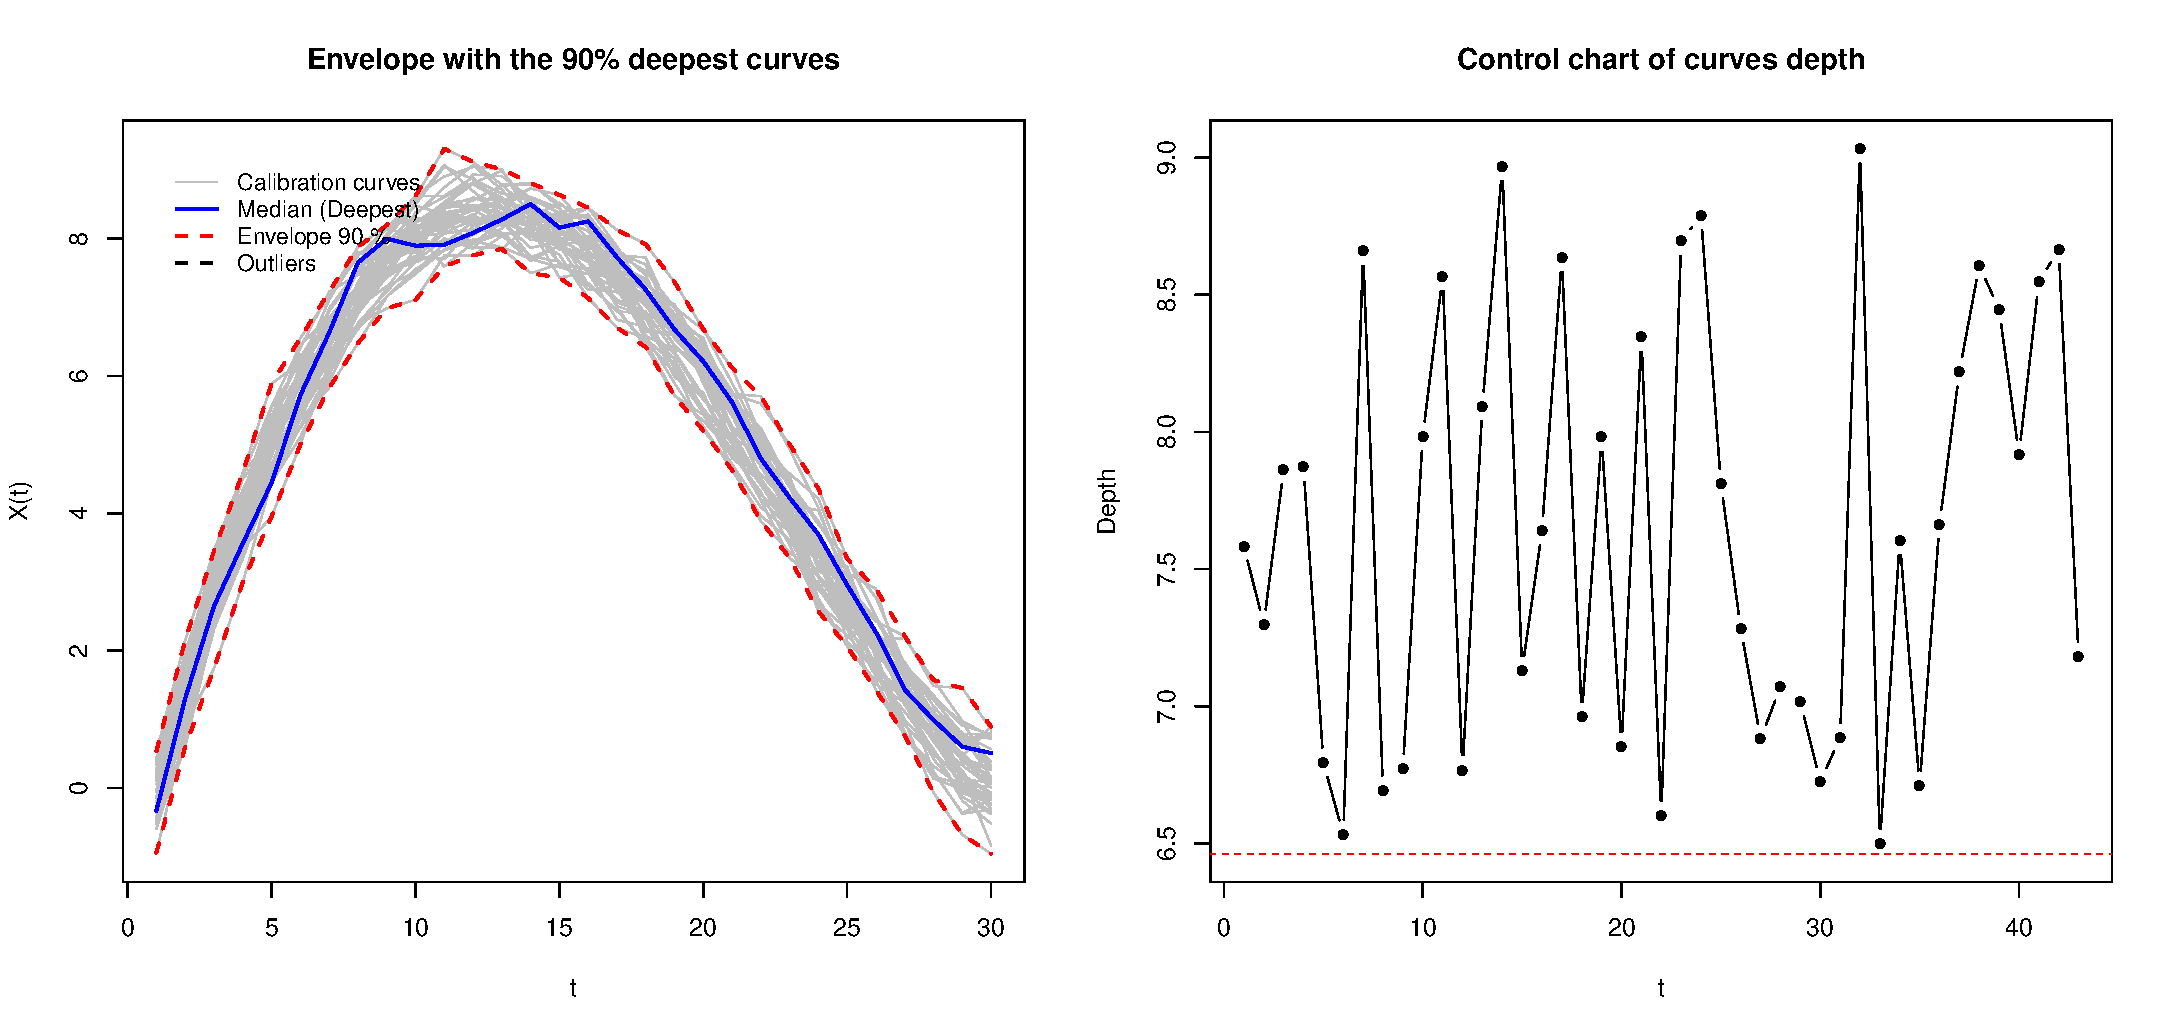
\includegraphics[width=\textwidth]{fda_3}
\caption{Results corresponding to the second iteration to obtain the in control calibration sample. Left panel: Original curves with the envelope composed of the 90\% of the deepest curves. Right panel: Control chart for the depths of the curves (the LCL has been estimated by bootstrap procedures at a signification level of 10\%.}
\label{fig:fda_3}
\end{center}
\end{figure}

\subsubsection{Estimating a Phase II control chart for functional data (monitoring)}

The next step is to perform the Phase II of process control. The monitoring phase is performed by the application of Phase II control charts for functional data based on multivariate nonparametric control charts. Firstly, a monitoring sample composed of 50 curves is simulated by the following code.

\begin{example}
R> mu_a<- 30 * tt^(3/2) * (1 - tt)
R> n_a <- 50
R> mdata_a<-matrix(NA,ncol=m,nrow=n_a)
R> for (i in 1:n_a) mdata_a[i,]<- mu_a+0.5*mvrnorm(mu = mu_a,Sigma = sigma )
\end{example}

The curves of the monitoring sample are defined with \code{fdqcd} format and a control chart for Phase II is developed by applying the \code{fdqcs.rank} function. It is composed by the following arguments, \code{fdqcs.rank(x, y = x, func.depth = depth.FM, alpha = 0.01, plot = TRUE, trim = 0.1, draw.control = NULL,...)}.

\begin{example}
R> fdchart_a <- fdqcd(mdata_a,"Monitoring curves")
R> phase2.chart <- fdqcs.rank(fdchart,fdchart_a)
R> plot(phase2.chart)
R> summary(phase2.chart)
\end{example}

Figure \ref{fig:fda_4} accounts for the FDA chart with the calibration sample and its envelope composed by the deepest curves. Moreover, the monitoring sample is also included and compared with the calibration sample by using the FDA chart. In addition, the Phase II rank control chart for functional data is shown including both calibration and monitoring samples or only the ranks corresponding to the monitoring sample. The second population that corresponds with the monitoring sample is identified by the control chart from the first monitored curve (panels below in Figure \ref{fig:fda_4}).

\begin{figure}[!htb]
\begin{center}
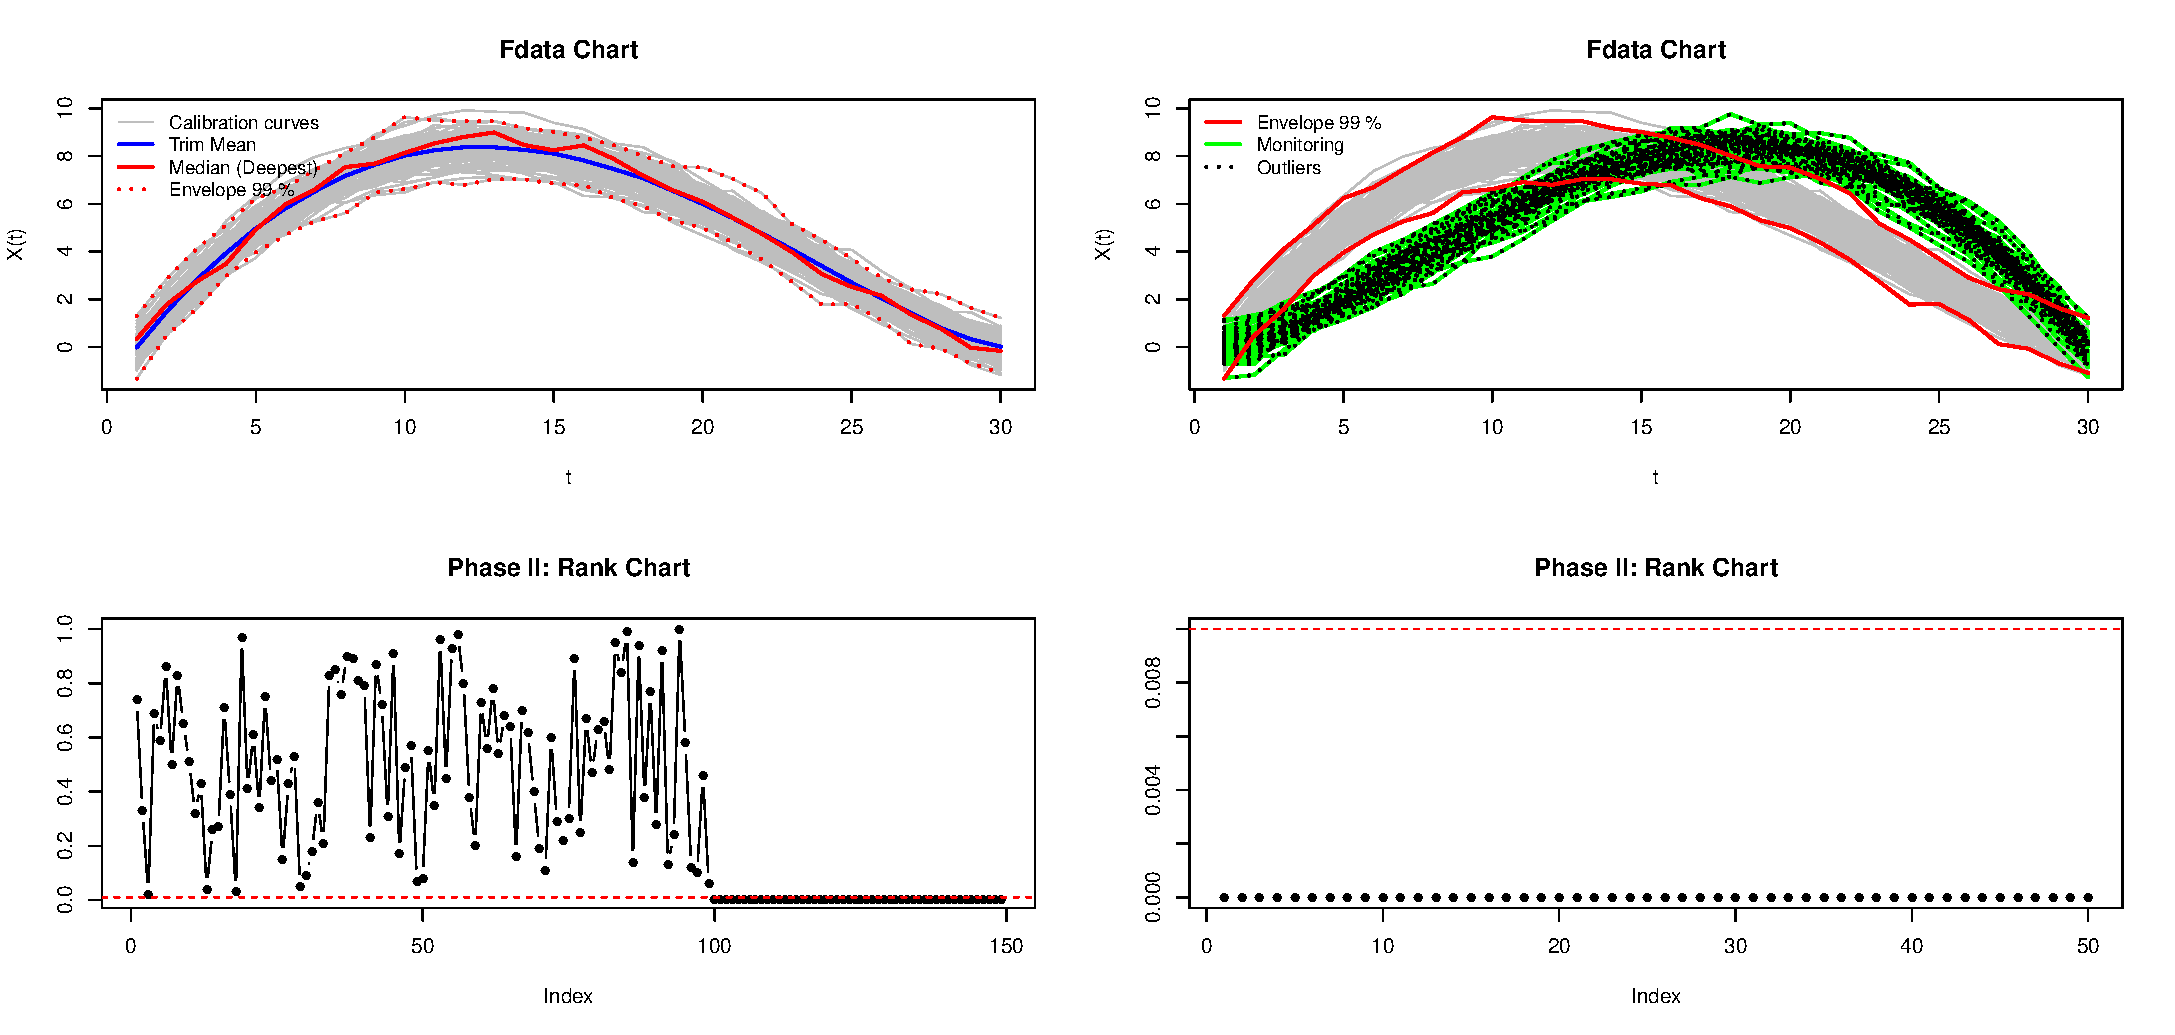
\includegraphics[width=\textwidth]{fda_4}
\caption{First row: the left and right panels show the FDA charts for the calibrating and monitoring samples with a signification level of 0.01. Second row: The left and right panels show the Phase II rank control chart for functional data, including calibration and monitoring sample (left panel) and only monitoring sample (right panel).}
\label{fig:fda_4}
\end{center}
\end{figure}






%-------------------------------------------
\section{Process capability analysis}
%-------------------------------------------

The analysis of the capability of a process in the case of statistical quality control is done through the calculation of the so-called capability. 
These indices measure whether a process is capable or not of meeting the corresponding technical specifications set by the customer, or the manufacturer, by comparing those with the natural variability of the CTQ variable that characterizes the process. 
The interpretation of these indices is associated with the result of this relation. 
Capability indices are generally calculated as the ratio between the length of the specification interval and the natural variability of the process in terms of $\sigma$. 
Large values of these indices mean that the corresponding process is capable of producing articles that meet the requirements of the client and manufacturers.
In other words, the larger the value of the capability index, the smaller the number of products outside the specification limits.

In this section, we describe the capability indices for processes whose underlying distribution is normal and not normal (exponential, Weibull, etc.).
However, it is important to note that the development of programming tools for nonparametric capability analysis is one of the main goals and contributions of the \CRANpkg{qcr} package. 
In addition to the estimation of capability indices, a graphical output is provided. 
Based on the proposal of \pkg{qualityTools} package, the \CRANpkg{qcr} graphical output for capability analysis includes a normality test for the CTQ variable, a Q-Q plot, a histogram with the theoretical Gaussian distribution density, parametric and nonparametric estimates of capability indices and a contour capability control chart.
In the following lines, parametric and nonparametric capability analysis utilities are described using different examples of applications.

%-------------------------------------------
\subsection{Assuming a normal distribution}
%-------------------------------------------

The most widely used capability indexes in the industry analyze the process capability under the assumptions of a 
stabilized process (in control) and a Gaussian distributed CTQ variable.
Table \ref{PCR} shows the main parametric (assuming Gaussian distribution) indices, namely  $C_p$, $C_{pk}$, $C_{pm}$, and $C_{pmk}$.

\citet{vannman1995unified} proposed a general formulation of these indices by an expression that depends on the non-negative parameters $u$ and $v$:
$$ C_p\left( u,v\right)= \frac{d-u\vert \mu - m\vert}{3\sqrt{\sigma^2+v\left( \mu - T\right)^2}},$$
whereby $d=(USL-LSL)/2$, $m=(LSL+USL)/2$, $USL$ is the upper specification limit, the $LSL$ is the lower specification limit, $\sigma$ is the theoretical standard deviation, $\mu$ accounts for the theoretical mean of the CTQ variable, and $T$ is the specification target (by default the mean between the $LSL$ and $USL$). 
The indices shown in Table \ref{PCR} are obtained from this expression just considering values of 0 or 1 for $u$ and $v$: $C_p\left( 0, 0\right)  = C_p$, $C_p\left( 1, 0\right)  = C_{pk}$, $C_p\left( 0, 1\right)  = C_{pm}$,
$C_p\left( 1, 1\right)  = C_{pmk}$.\\

\begin{table}[!htb]
\centering

\begin{tabular}{|l|l|}
\hline
Potential capability & $\hat{C}_p = \frac{USL - LSL} {6 \hat{\sigma}}$ \\ \hline
\begin{tabular}[c]{@{}l@{}}Actual capability with respect\\ to the specification limits\end{tabular} & \begin{tabular}[c]{@{}l@{}}$\hat{C}_{p,lower} = \frac{\hat{\mu} - LSL}{3 \hat{\sigma}}$\\ \\ $ \hat{C}_{p,upper} = \frac{USL - \hat{\mu}}{3 \hat{\sigma}}$\\ \\ $ \hat{C}_{pk} = \min \left[ \frac{USL - \hat{\mu}}{3 \hat{\sigma}}, \frac{\hat{\mu} - LSL}{3 \hat{\sigma}} \right] $ \end{tabular} \\ \hline
\begin{tabular}[c]{@{}l@{}}Shifting of the mean with\\ respect to the target\end{tabular}
& $\hat{C}_{pm} = \frac{ \hat{C}_p } { \sqrt{ 1 + \left ( \frac{\hat{\mu} - T} {\hat{\sigma}} \right )^2 } }$    \\ \hline
\begin{tabular}[c]{@{}l@{}}$C_{pk}$ correction for detecting\\ deviations with respect to the target\end{tabular} & $\hat{C}_{pkm} = \frac{ \hat{C}_{pk} } { \sqrt{ 1 + \left ( \frac{\hat{\mu} - T} {\hat{\sigma}} \right )^2 } }$  \\ \hline
\end{tabular}
\caption{PCR from first to fourth generation, $USL$ is the upper specification limit, $LSL$ is the lower specification limit, $\mu$ is the real mean, $\hat{\mu}$ is the estimated mean, and $\hat{\sigma}$ is the estimated standard deviation. }
\label{PCR}
\end{table}

The piston rings data set is used to illustrate the calculation of the capability indices using the \code{qcs.cp()} function based on the expressions previously described in Table \ref{PCR}. From the statistics obtained from the $\bar{x}$ control chart of pistonrings dataset, the $\gamma$ and $\beta$ values are estimated, and the corresponding capability index is computed.
\begin{example}
R> data("pistonrings")
R> xbar <- qcs.xbar(pistonrings[1:125, ], plot = FALSE)
R> limits <- c(lsl = 73.99, usl = 74.01)
R> # qcs.cp(object = xbar, parameters = c(0, 0), limits = limits, 
R> #        contour = FALSE)
R> # qcs.cp(object = xbar, parameters = c(1, 0), limits = limits, 
R> #        contour = FALSE)
R> # qcs.cp(object = xbar, parameters = c(0, 1), limits = limits, 
R> #        contour = FALSE)
R> qcs.cp(object = xbar, parameters = c(1, 1), limits = limits, 
+         contour = FALSE)
\end{example}
\begin{example}
     Cpmk delta.usl gamma.usl 
   0.2984    0.1176    0.9785 
\end{example}

Consequently, the obtained results are $ C_p=0.3407$, $C_{pk}=0.3006$, $C_{pm}=0.3382$, and $ C_{pmk}=0.2984$, respectively. The argument \code{parameters} account for $u$ and $v$ values, while \code{object} is the type of control chart from which the $\sigma$ is estimated, \code{limits} are the specification control limits, and \code{contour} is the parameter that indicates when the process capability contour chart is plotted.

%-------------------------------------------
\subsection{Process capability plot}
%-------------------------------------------
In \citet{vannman2001graphical} and \citet{deleryd1999process}, a graphical method (based on common capability indices) to analyze the capability of a process is proposed. 
The goal of using this type of plot (if compared with respect to only capability indices calculation) is to provide immediate information of the location and spread of the CTQ feature and about the capability to meet the specifications of the corresponding process. 
When using this chart, a process will be $capable$ if the process capability index is higher than a certain value $k$, with $k> 1$. 
The most used values for $k$ are $k = 1$, $k = 4/3$, or $k = 5/3$, even 2 at a Six Sigma level, taking into account the usual index limits for which a process could be assumed capable.  
It will also be assumed that the target value matches the center of the specification interval, that is,  $T = \frac{\left( USL + LSL\right)}{2} = m$. 
Then, one of the indices defined by the $C_p\left( u,v\right)$ family is used, e.g., $C_{pk}$ or $C_{pm}$,
and the process will be defined as capable if $C_p\left( u, v \right)> k$, given the values of $u$, $v$, and $k$. 
Also note that if $\mu = T$, all the $C_p\left( u, v\right)$ indices are defined by the same expression as the $C_p$. 
Moreover, different setting for $u$, $v$, and $k$ impose different constraints on the process parameters $\left( \mu, \sigma \right)$. 
This can be easily seen through a process capability plot. 
This graph is a contour plot of $C_p\left( u, v\right)  = k$ as a function of $\mu$ and $\sigma$, but it can also be defined as a function of $\delta$ and $\gamma$, with $\delta = \frac{\mu - T}{d}$ and $\gamma = \frac{\sigma}{d}$. 
The contour line is obtained by rewriting the index $C_p\left( u,v\right)$ as a function of $\delta$ and $\gamma$ as follows $ C_p\left( u,v\right)= \frac{1-u\vert \delta \vert}{3\sqrt{\gamma^2+v\left( \delta \right)^2}}$. 
Therefore, the $C_p\left( u,v\right) = k$ equation is solved, plotting $\gamma$ depending on the values of $\delta$. 
The resulting expressions are:
$$ \gamma = \sqrt{\frac{\left( 1-u\vert\delta\vert\right)}{9k^2}-v\delta^2}, \; \vert\delta\vert \leq \frac{1}{u+3k\sqrt{v}}, \; \left( u,v\right) \neq \left(0,0 \right)$$
When $u = v = 0$, that is, when we consider the index $C_p=k$, we have $\gamma = \frac{1}{3k}$ and $\vert\delta\vert \leq 1$. 
It is important to highlight that the $\gamma$-axis accounts for the process spread, whereas the $\delta$-axis accounts for the process location. 
The values of the parameters $\mu$ and $\sigma$ which provide values $\left( \delta,\gamma\right)$ within the region bounded by the contour line $C_p\left(u, v\right) = k$ and the $\delta$-axis will provide a larger $C_p\left(u, v\right)$ value than $k$, leading a capable process. 
Furthermore, values of $\mu$ and $\sigma$ which provide values $\left( \delta,\gamma\right)$ outside this region will provide a value $C_p\left(u, v\right)$ smaller than $k$, i.e., a non-capable process. 
In the case of the process not being capable, this type of plot is useful to understand if the corrective actions have to be performed to decrease the process spread, or the process location (deviation with respect to target), or even when both changes are needed to improve the process capability. 
This can be observed by observing the distance with respect to the $x$ and $y$-axis. 
Below are some examples of capability plot application which can be generated through the application of the \code{qcs.cp} function with \code{contour=TRUE} and \code{k=1} (default values):
\begin{example}
R> oldpar <- par(mfrow = c(2, 2))
R> qcs.cp(object = xbar, parameters = c(0, 0), limits = limits, 
+         ylim = c(0, 1))
R> qcs.cp(object = xbar, parameters = c(1, 0), limits = limits,  
+         ylim = c(0, 1))
R> qcs.cp(object = xbar, parameters = c(0, 1), limits = limits,  
+         ylim = c(0, 1))
R> qcs.cp(object = xbar, parameters = c(1, 1), limits = limits,  
+         ylim = c(0, 1))
R> par(oldpar)
\end{example}
The result is shown in Figure~\ref{fig:cpplot}. In all the cases, the points in red are out of the area defined by the line in blue and the $\delta$ axis. 
Thus, the corresponding process is not capable, no matter the capability index that is used.
In any case, note that the $C_{p}$ index is useless in identifying non-capable processes due to location shifts 
with respect to the target. 
In the same way, the $C_{pk}$ index assumes as capable processes that are far from the target as long as they were close to the specification limits (as shown in Figure~\ref{fig:cpplot}). 
Thus, the use of the $C_{pm}$ and $C_{pmk}$ are recommended due to they take into account both shifts from the target and the spread. 
In the present case, the process is not capable due to the spread rather than the target shift.
Therefore, the process changes could be due to decreases in the variability process.
\begin{figure}[!htb]
\begin{center}
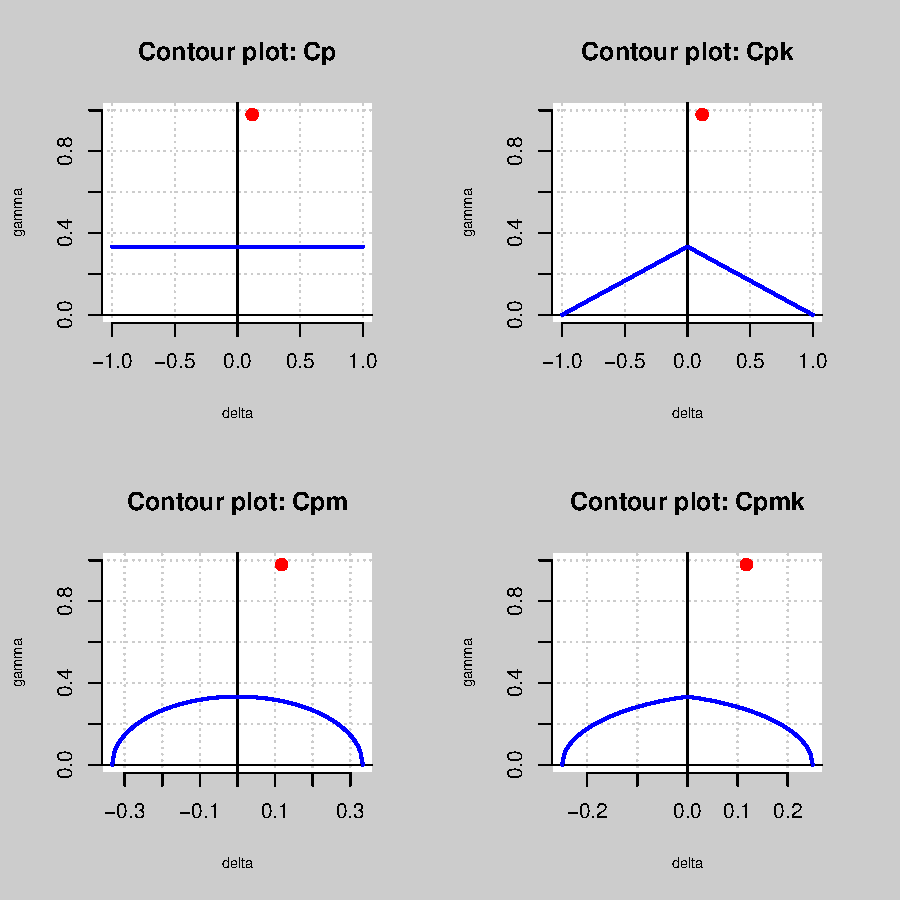
\includegraphics[width=0.8\textwidth]{article-cpplot-plot}
\caption{Process capability plots using the $C_p$, $C_{pk}$, $C_{pm}$, and $C_{pmk}$ indexes.}
\label{fig:cpplot}
\end{center}
\end{figure}

%-------------------------------------------
\subsection{Estimated process capability plot}
%-------------------------------------------


In practice, the process parameters are unknown and we need to estimate them.  We can perform a decision rule based on the sample statistics that provide a sample estimate of the capability index and, finally the so called estimated process capability plot, also called  $\gamma^*-\delta^*$ plot \citep{deleryd1999process}. 
It allows us to decide whether a process is capable or not assuming that $\mu$ and $\sigma$ parameters are unknown and estimated by 
$\hat{\mu}=\bar{X}$ and $\hat{\sigma}^2=\frac{1}{n}\sum_{i=1}^n{X^2_i-\bar{X}^2}$. 
They are the maximum likelihood estimators when the CTQ variable of the process is normally distributed, and $ X_1,X_2,\dots,X_n$ is a random sample of a normal distribution with $\mu$ mean and $\sigma^2$ variance.\\
The \CRANpkg{qcr} package only provides the $\gamma^*-\delta^*$ plot corresponding to the $C_{pm}$ index taking into account that the other capability indices do not consider shifts from the target value in their calculations. 
For the general case, see the work of \cite{vannman2001graphical}. 
In order to obtain an appropriate decision rule for the case of $C_{pm}$ index, we test the hypotheses $H_0 : C_{pm} \leq k_0$ versus $H_1 : C_{pm} > k_0$, using
$$\hat{C}_{pm}= \frac{d}{3\sqrt{\hat{\sigma}^2+\left( \hat{\mu} - T\right)^2}}$$ 
as test statistic. 
The null hypothesis will be rejected if $\hat{C}_{pm} > c_{\alpha}$, where the constant $c_{\alpha}$ is determined by previously defining a signifition test level $\alpha$ . 
\citet{vannman2001graphical} showed that the null hypothesis $H_0:C_{pm} \leq k_0$ can be reduced to $H_0:C_{pm}=k_0$. 
Thus, for given values of $\alpha$ and $n$, the process will be considered capable if $\hat{C}_{pm} > c_{\alpha}$, with $c_{\alpha} > k_0$. 
\citet{hubele2004effect} proved that, when the $C_{pm}$ index is used, the critical value for a given $\alpha$ is obtained as 
$$c_{\alpha}=k_0\sqrt{\frac{n}{\chi^2_{\alpha,n}}},$$
where $\chi^2_{\alpha,n}$ is the quantile $\alpha$ of a $\chi^2$ distribution with $n$ degrees of freedom.
The \CRANpkg{qcr} package includes the \code{qcs.hat.cpm()} function to obtain both the theoretical capability plot and the estimated capability plot from sample statistics. 
Among other options, the user can indicate the control chart from which the estimates $\hat{\mu}$ and $\hat{\sigma}$ are obtained (alternatively, $\hat{\mu}$ and $\hat{\sigma}$ can be introduced through \code{mu} and \code{std.dev}), and the specification limits using \code{limits}. 
Furthermore, the signification level and the capability limit can be modified, as they are set to $\alpha=0.05$ and $k_0=1$ by default. 
The following code illustrates its application to \code{pistonrings} data. 
\begin{example}
R> xbar <- qcs.xbar(pistonrings[1:125, ], plot = FALSE)
R> limits <- c(lsl = 73.99, usl = 74.01)
R> # qcs.hat.cpm(object = xbar, limits = limits, ylim = c(0,1))
R> mu <- xbar$center
R> std.dev <- xbar$std.dev
R> qcs.hat.cpm(limits = limits, mu = mu, std.dev = std.dev, ylim = c(0,1))
\end{example}
The result is shown in Figure \ref{fig:cpplot2}. 
The contour line corresponding to the capability region obtained from the capability index sample is always more restrictive than the corresponding theoretical one.
\begin{figure}[!htb]
\begin{center}
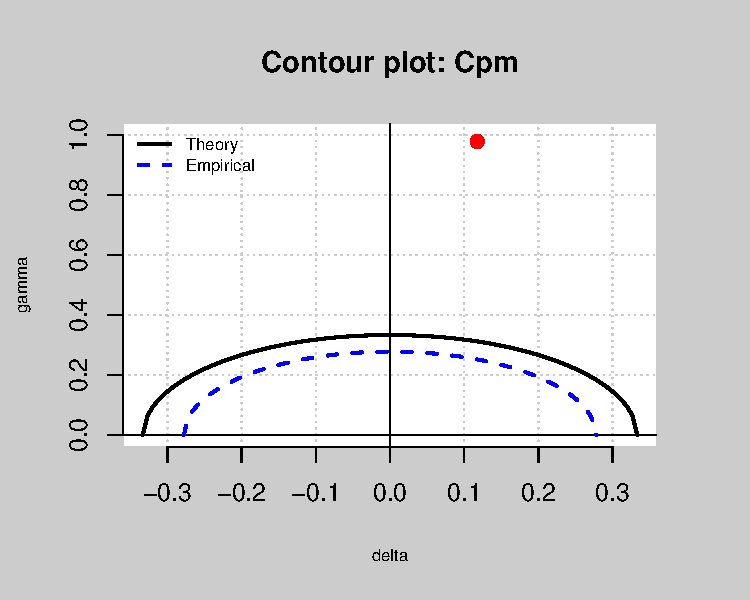
\includegraphics[width=0.8\textwidth]{article-cpplot2-plot}
\caption{Comparison between theorical and estimated process capability plots.}
\label{fig:cpplot2}
\end{center}
\end{figure}

%-------------------------------------------
\subsection{Nonparametric capability analysis}
%-------------------------------------------

Traditional assumptions about data such as normality or independence are frequently violated in many real situations. 
Thus, in scenarios in which assumptions of normality are not verified, the indices defined in the previous sections are not valid. 
\citet{pearn1997practical} and \citet{tong1998lower} proposed generalizations of $C_p\left(u, v\right)$ for the case of arbitrary distributions of data
$$ C_{Np}\left( u,v\right)= \frac{d-u\vert M - m\vert}{3\sqrt{\left(\frac{F_{99.865}-F_{0.135}}{6} \right)^2+v\left( M - T\right)^2}},$$
where $F_{\alpha}$ is the percentile $\alpha$\% of the corresponding distribution and $M$ the median of the process. 
However, the distribution of the underlying process is always unknown. 
\cite{chang1994pci} calculated estimates for $F_{99.865}$, $F_{0.135}$ and $M$ based on the sample percentiles.

\citet{pearn1997practical} proposed the following estimator
$$ \hat{C}_{Np}\left( u,v\right)= \frac{d-u\vert \hat{M} - m\vert}{3\sqrt{\left(\frac{U_p-L_p}{6} \right)^2+v\left( \hat{M} - T\right)^2}}$$
where $U_p$ is an estimator for $F_{99.865}$, $L_p$ is an estimator for $F_{0.135}$, and $\hat{M}$ is an estimator for $M$, obtained from the tables developed by \cite{gruska1989non}. 

The \code{qcs.cpn()} function of \CRANpkg{qcr} calculates $C_{Np}$, $C_{Npk}$, $C_{Npm}$, and $C_{Npmk}$ using the formulation described by \citet{tong1998lower}. 
The code that illustrates its use is shown below. 
To obtain the nonparametric capability indices it is necessary to indicate the $u$ and $v$ parameters.
\begin{example}
R> xbar <- qcs.xbar(pistonrings[1:125, ], plot = FALSE)
R> limits <- c(lsl = 73.99, usl = 74.01)
R> # x <- xbar$statistics[[1]]
R> # median <- median(x)
R> # q = quantile(x, probs = c(0.00135, 0.99865)) # c(lq, uq)
R> # qcs.cpn(parameters = c(0, 0), limits = limits, median = median, q = q)
R> # qcs.cpn(object = xbar, parameters = c(0, 0), limits = limits)
R> # qcs.cpn(object = xbar, parameters = c(1, 0), limits = limits)
R> # qcs.cpn(object = xbar, parameters = c(0, 1), limits = limits)
R> qcs.cpn(object = xbar, parameters = c(1, 1), limits = limits)
\end{example}
\begin{example}
 CNpmk 
0.9015 
\end{example}
Thus, the values obtained are $C_{Np}=1.0082$, $C_{Npk}=0.9275$, $C_{Npm}=0.9799$ and $C_{Npmk}=0.9015$. 
If a capability limit of $k=1$ or $k=1.33$ is assumed, we can infer that the process is not actually capable to meet the customers or 
manager's requirements.

%-------------------------------------------
\subsection{Tools for a comprehensive processs capability analysis}
%-------------------------------------------

Function \code{qcs.ca()} provides a comprehensive information of the capability of a process, summarized through a graphical output. This function calculates the process capability indices $C_p$, $C_{pk}$, $C_{pL}$, $C_{pU}$, $C_{pm}$, $C_{pmk}$ from a \code{qcs}  object, assuming a Gaussian distribution. 
Moreover, it computes confidence limits for $C_p$ using the method described by \citet{chou1990lower}. 
Approximate confidence limits for $C_{pl}$, $C_{pu}$, and $C_{pk}$ are also estimated using the method described in \citet{bissell1990reliable}, while the confidence limits for $C_{pm}$ are based on the approximated method of \citet{boyles1991taguchi} that assumes the target is the mean of the specification limits. 
Moreover, the $C_{Np}$, $C_{Npk}$, $C_{Npm}$, and $C_{Npmk}$ nonparametric capability indices are also obtained. 
There is also a specific box within the summary plot that shows the proportion of observations and expected observations under the Gaussian assumption out of the specification limits (nonconforming observations).
Further, a histogram of the data sample is provided, in addition to the corresponding Gaussian density curves obtained from the sample estimates (one per standard deviation estimate procedure).
They are displayed along with the specification limits, a quantile-quantile plot for the specified distribution, and a process capability plot obtained from the $C_{pm}$ index (both using theoretical and sample alternatives). 
In order to describe the \code{qcs.ca()} performance, the following code corresponds to the analysis of the first 125 observations of the \code{pistonrings} dataset (the corresponding output is shown in Figure \ref{fig:caplot}).

\begin{example}
R> qcs.ca(xbar, limits = c(lsl = 73.99, usl = 74.01))
\end{example}
\begin{example}
Process Capability Analysis

Call:
qcs.ca(object = xbar, limits = c(lsl = 73.99, usl = 74.01))

Number of obs = 125          Target = 74
       Center =  74               LSL =  73.99
       StdDev =  0.009785         USL =  74.01

Paremetric Capability indices:

       Value    0.1%   99.9%
Cp    0.3407  0.2771  0.4065
Cp_l  0.3807  0.2739  0.4875
Cp_u  0.3006  0.2021  0.3991
Cp_k  0.3006  0.1944  0.4068
Cpm   0.3382  0.2749  0.4038


Non parametric Capability indices:

        Value
CNp    1.0082
CNpK   0.9275
CNpm   0.9799
CNpmk  0.9015


PPM:

         Exp<LSL 1.267e+07       Obs<LSL 0
         Exp>USL 1.836e+07       Obs>USL 8e+05
       Exp Total 3.103e+07     Obs Total 8e+05

Test:


	Anderson Darling Test for normal distribution

data:  xbar 
A = 0.1399, mean = 74.001, sd = 0.005, p-value = 0.9694
alternative hypothesis: true distribution is not equal to normal 
\end{example}

%
\begin{figure}[H]
\begin{center}
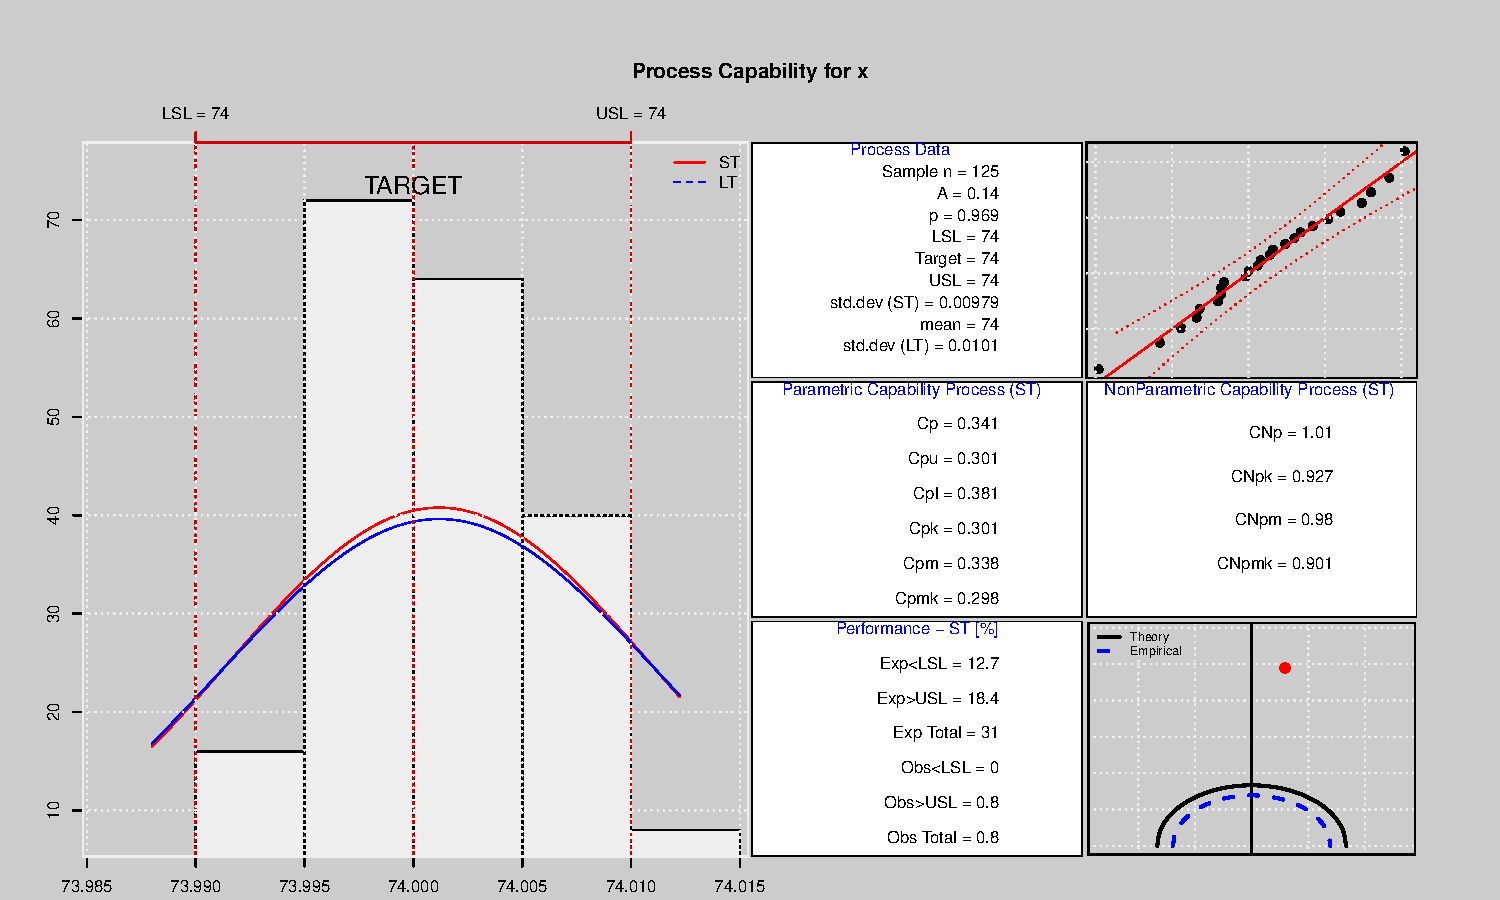
\includegraphics[width=\textwidth]{article-caplot-plot}
\caption{A complete analysis of the process capability.}
\label{fig:caplot}
\end{center}
\end{figure}

%-------------------------------------------
 \section{Conclusions}
%-------------------------------------------

The \CRANpkg{qcr} package has been developed to provide users with a comprehensive set of functions that manage statistical process control, ranging from univariate parametric analysis to multivariate and FDA nonparametric statistics.
This package includes the main types of control charts and capability indices.
It combines the main features of reputed SQC packages in R such as \CRANpkg{qcc} and \pkg{qualityTools} with the proposal of a new graphical appearance and the implementation of new SQC tools with increasing importance in Industry 4.0 such as multivariate and nonparametric analysis.\\
In addition to some utilities provided by reference R packages such as \CRANpkg{qcc}, \CRANpkg{SixSigma}, and \pkg{qualityTools}, \CRANpkg{qcr} implements very important statistical techniques of Control and Analysis tasks of the Six Sigma procedure that are not included in other libraries. 
In the case of multivariate control charts, these tools are the MEWMA and MCUSUM multivariate control charts, on the one hand, and the $r$, $Q$ and $S$ nonparametric control charts based on data depth, on the other hand. In addition, Phase I and Phase II control charts for functional data (monthly, daily, hourly curves) based on functional data depth, bootstrap procedures, and nonparametric rank charts have also been implemented in the \CRANpkg{qcr} package. These control charts for functional data provide tools to control and improve processes when their CTQ variables are obtained as hourly, monthly, daily, yearly smooth curves.\\
It is also very important to note that \CRANpkg{qcr} provides functions to perform nonparametric capability analysis. 
In addition, the new implementation of the process capability plots for the main parametric capability indices allows us to analyze if improvements in process spread or/and process location are needed to obtain a capable process. 
The comparison between suppliers, machines, etc., is enabled through capability plots.\\
%The \texttt{qcr} package also includes an automatic way to delete out of control states in the process of chart natural control limits estimation.
All these utilities intend to make \CRANpkg{qcr} a useful tool for users of a wide variety of industries, providing a competitive alternative to commercial software.

%% -- Optional special unnumbered sections -------------------------------------
% %-------------------------------------------
% \section*{Computational details}
% %-------------------------------------------
% 
% The results in this paper were obtained using
% \texttt{R}~3.5.1 with the
% \texttt{qcr}~1.0 package. \texttt{R} itself
% and all packages used are available from the Comprehensive
% \texttt{R} Archive Network (CRAN) at
% \url{https://CRAN.R-project.org/}.


%-------------------------------------------
\section*{Acknowledgments}
%-------------------------------------------

The work of Salvador Naya, Javier Tarr\'io-Saavedra, Miguel Flores and Rub\'en Fern\'andez-Casal has been supported by MINECO grant MTM2017-82724-R,  and by the Xunta de Galicia (Grupos de Referencia Competitiva ED431C-2020-14 and Centro de Investigaci\'on del Sistema universitario de Galicia ED431G 2019/01), all of them through the ERDF. The research of Miguel Flores has been partially supported by Grant PII-DM-002-2016 of Escuela Polit\'ecnica Nacional of Ecuador. In addition, the research of Javier Tarr\'io-Saavedra has been also founded by the eCOAR project (PC18/03) of CITIC. The authors thank Mateo Larco and Bibiana Santiso for their valuable help with the English edition.
\bibliography{RJreferences}


\address{Miguel Flores\\
  MODES, SIGTI, ADIAAC, Departamento de Matem\'aticas, Escuela Polit\'ecnica Nacional\\
  170517 Quito\\
  Ecuador\\
  0000-0002-7742-1247\\
  \email{miguel.flores@epn.edu.ec}}

\address{Rub\'en Fern\'andez-Casal\\
  MODES, CITIC, Universidade da Coru\~{n}a\\
  Facultade de Inform\'atica, Campus de Elvi\~{n}a, A Coru\~{n}a\\
  Spain\\
  0000-0002-5785-3739\\
  \email{ruben.fcasal@udc.es}}

\address{Salvador Naya\\
  MODES, CITIC, ITMATI, Universidade da Coru\~{n}a\\
  Escola Polit\'ecnica Superior, Mendiz\'abal s/n, Ferrol \\
  Spain\\
  0000-0003-4931-9859\\
  \email{salva@udc.es}}
	
	\address{Javier Tarr\'io-Saavedra\\
  MODES, CITIC, Universidade da Coru\~{n}a\\
  Escola Polit\'ecnica Superior, Mendiz\'abal s/n, Ferrol \\
  Spain\\
  0000-0003-4931-9859\\
  \email{javier.tarrio@udc.es}}
